
\newcommand{\pagex}{
\heading{Objectius del tema:}
\vspace{0.25cm}

{
\fontsize{10.5}{12.8}\selectfont
1. Utilitzar els nombres reals, les seves operacions i propietats, per recollir, transformar i intercanviar informació, estimant, valorant i representant els resultats en contextos de resolució de problemes.

1.1. Reconeix els diferents tipus de nombres (reals i complexos) i els utilitza per representar i interpretar adequadament informació quantitativa.

1.2. Realitza operacions numèriques amb eficàcia, emprant càlcul mental, algoritmes de llapis i paper, calculadora o eines informàtiques.

1.3. Utilitza la notació numèrica més adequada a cada context i justifica la seva idoneïtat.

1.4. Obté fites d’error i estimacions en els càlculs aproximats que realitza valorant i justificant la necessitat d’estratègies adequades per minimitzar-les.

1.5. Coneix i aplica el concepte de valor absolut per calcular distàncies i tractar desigualtats.

1.6. Resol problemes en què intervenen nombres reals i la seva representació i interpretació en la recta real.

}
}

 

\newcommand{\pagexvi}{
	\heading{Objectius del tema:}
	\vspace{0.25cm}
	
	{
		\fontsize{10.5}{12.8}\selectfont
	 4. Analitzar, representar i resoldre problemes plantejats en contextos reals, utilitzant recursos algebraics (equacions, inequacions i sistemes) i interpretant críticament els resultats.
	 
4.1. Formula algebraicament les restriccions indicades en una situació de la vida real, estudia i classifica un sistema d’equacions lineals plantejat (com a màxim de tres equacions i tres incògnites), el resol mitjançant el mètode de Gauss, en els casos que sigui possible, i l’aplica per resoldre problemes.

4.2. Resol problemes en els quals es necessiti el plantejament i resolució d’equacions (algebraiques i no algebraiques) i inequacions (primer i segon grau), i interpreta els resultats en el context del problema.
		
	}
}

\newcommand{\pagexxxi}{
	\heading{Objectius del tema:}
	
	\vspace{0.25cm}
	{
		\fontsize{10.5}{12.8}\selectfont
		1. Reconèixer i treballar amb els angles en radiants tractant amb facilitat les raons trigonomètriques d’un angle, del seu doble i meitat, així com les transformacions trigonomètriques usuals.
		
1.1. Coneix les raons trigonomètriques d’un angle,el seu doble i meitat, així com les de l’angle suma i diferència d’uns altres dos.

2. Utilitzar els teoremes del sinus, cosinus i tangent i les fórmules trigonomètriques usuals per resoldre equacions trigonomètriques, així com aplicar-les en la resolució de triangles directament o com a conseqüència de la resolució de problemes geomètrics del món natural, geomètric o tecnològic.

2.1. Resol problemes geomètrics del món natural, geomètric o tecnològic, utilitzant els teoremes del sinus, del cosinus i de la tangent i les fórmules trigonomètriques usuals.

		
	}
}

 

\newcommand{\pagelix}{
	\heading{Objectius del tema:}
	\vspace{0.25cm}
	{
		\fontsize{10.5}{12.8}\selectfont
		
		1. Identificar funcions elementals, donades a través d’enunciats, taules o expressions algebraiques, que descriguin una situació real, i analitzar, qualitativament i quantitativament, les seves propietats, per representar-les gràficament i extreure informació pràctica que ajudi a interpretar el fenomen de què es deriven.
		
1.1. Reconeix analíticament i gràficament les funcions reals de variable real elementals.

1.2. Selecciona de manera adequada i raonada eixos, unitats, domini i escales, i reconeix i identifica els errors d’interpretació derivats d’una mala elecció.

1.3. Interpreta les propietats globals i locals de les funcions, comprovant els resultats amb l’ajuda de mitjans tecnològics en activitats abstractes i problemes contextualitzats.

1.4. Extreu i identifica informacions derivades de l’estudi i anàlisi de funcions en contextos reals.

3. Valorar les aplicacions del nombre e i dels logaritmes utilitzant les seves propietats en la resolució de problemes extrets de contextos reals.

3.1. Aplica correctament les propietats per calcular logaritmes senzills en funció d’altres coneguts.

3.2. Resol problemes associats a fenòmens físics, biològics o econòmics mitjançant l’ús de logaritmes i les seves propietats.

	}
}

\newcommand{\pagelxxiii}{
	\heading{Objectius del tema:}
	
	\vspace{0.25cm}
	{
		\fontsize{10.5}{12.8}\selectfont
		2. Utilitzar els conceptes de límit i continuïtat d’una funció i aplicar-los en el càlcul de límits i l’estudi de la continuïtat d’una funció en un punt o un interval.
		
2.1. Comprèn el concepte de límit, fa les operacions elementals per calcular-lo, i aplica els processos per resoldre indeterminacions.

2.2. Determina la continuïtat d’una funció en un punt a partir de l’estudi del seu límit i del valor de la funció, per extreure conclusions en situacions reals.

2.3. Coneix les propietats de les funcions contínues, i representa la funció en un entorn dels punts de discontinuïtat.

	}
}


\newcommand{\pagelxxxvi}{
	
	\vso
	
	\heading{Objectius del tema:}
	
	\vspace{0.25cm}
	{
		\fontsize{10.5}{12.8}\selectfont
		3. Aplicar el concepte de derivada d’una funció en un punt, la seva interpretació geomètrica i el càlcul de derivades a l’estudi de fenòmens naturals, socials o tecnològics i a la resolució de problemes geomètrics.
		
3.1. Calcula la derivada d’una funció usant els mètodes adequats i l’empra per estudiar situacions reals i resoldre problemes.

3.2. Deriva funcions que són composició de diverses funcions elementals mitjançant la regla de la cadena.

3.3. Determina el valor de paràmetres perquè es verifiquin les condicions de continuïtat i derivabilitat d’una funció en un punt.

4. Estudiar i representar gràficament funcions obtenint informació a partir de les seves propietats i extraient informació sobre el seu comportament local o global.
	}
}


\newcommand{\pagecxx}{
	\heading{Objectius del tema:}
	
	\vspace{0.25cm}
	{
		\fontsize{10.5}{12.8}\selectfont
		4. Interpretar analíticament diferents situacions de la geometria plana elemental, obtenint les equacions de rectes i utilitzar-les, per resoldre problemes d’incidència i càlcul de distàncies.
		
4.1. Calcula distàncies entre punts i d’un punt a una recta, així com angles entre dues rectes.

4.2. Obté l’equació d’una recta en les seves diverses formes, identificant en cada cas els seus elements característics.

4.3. Reconeix i diferencia analíticament les posicions relatives de les rectes.


	}
}


\newcommand{\pagecxxx}{
	\heading{Objectius del tema:}
	
	\vspace{0.25cm}
	{
		\fontsize{10.5}{12.8}\selectfont
		5. Tractar el concepte de lloc geomètric en el pla. Identificar les formes corresponents a alguns llocs geomètrics usuals, estudiant les seves equacions reduïdes i analitzant les seves propietats mètriques.
		
5.1. Coneix el significat de lloc geomètric, identificant els llocs més usuals en geometria plana així com les seves característiques.

5.2. Fa investigacions utilitzant programes informàtics específics en els quals cal seleccionar, estudiar posicions relatives i fer interseccions entre rectes i les diferents còniques estudiades.
	}
}


\newcommand{\pagecxliii}{
	\heading{Objectius del tema:}
	
	\vspace{0.25cm}
	{
		\fontsize{10.5}{12.8}\selectfont
	 1. Descriure i comparar conjunts de dades de distribucions bidimensionals
	 
1.1. Elabora taules bidimensionals de freqüències a partir de les dades d’un estudi estadístic, amb variables discretes i contínues.

1.2. Calcula i interpreta els paràmetres estadístics més usuals en variables bidimensionals.

1.3. Calcula les distribucions marginals i diferents distribucions condicionades a partir d’una taula de contingència, així com els seus paràmetres (mitjana, variància i desviació típica).

1.4. Decideix si dues variables estadístiques són o no dependents a partir de les seves distribucions condicionades i marginals.

1.5. Usa adequadament mitjans tecnològics per organitzar i analitzar dades des del punt de vista estadístic, calcular paràmetres i generar gràfics estadístics.

2. Interpretar la possible relació entre dues variables i quantificar la relació lineal.
 
2.1. Distingeix la dependència funcional de la dependència estadística i estima si dues variables són o no estadísticament dependents mitjançant la representació del núvol de punts.

2.2. Quantifica el grau i sentit de la dependència lineal entre dues variables mitjançant el càlcul i interpretació del coeficient de correlació lineal.

2.3. Calcula les rectes de regressió de dues variables i obté prediccions a partir d’elles.

2.4. Avalua la fiabilitat de les prediccions obtingudes a partir de la recta de regressió mitjançant el coeficient de correlació lineal.
 
	}
}

\newcommand{\pagecxxxvi}{
	\newpage
	
	\vspace*{\fill}
	
	\heading{Aplicacions de les còniques}
	
	\begin{center}
	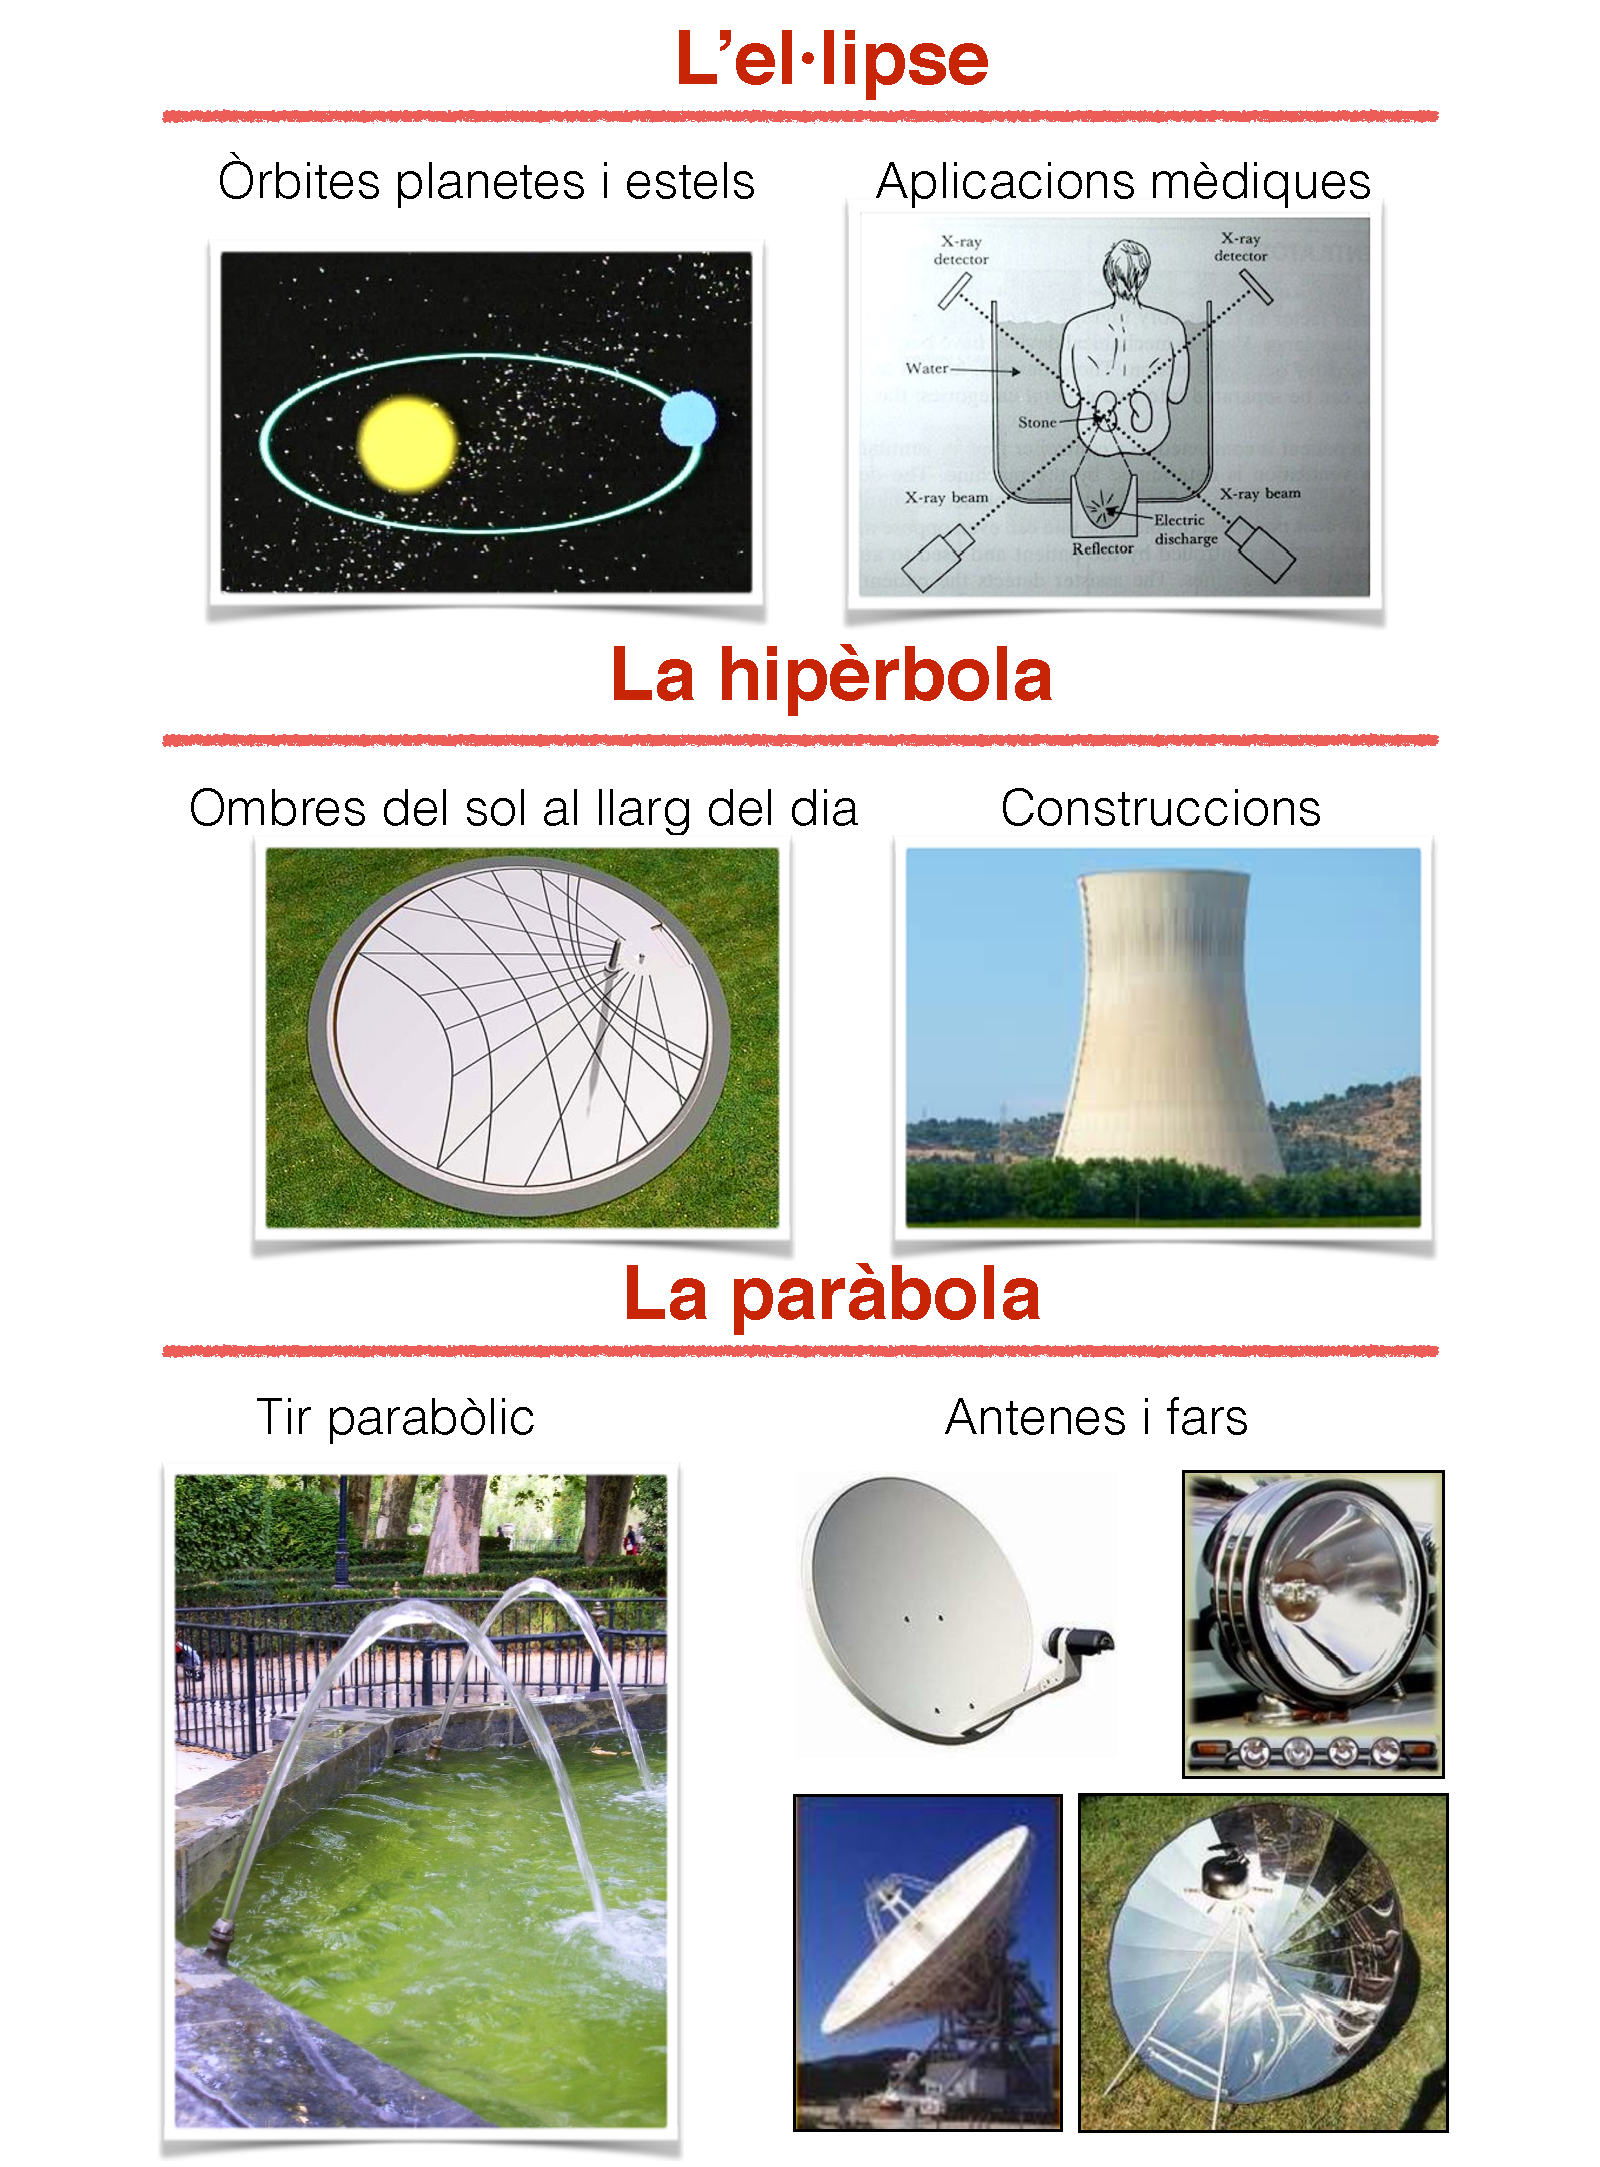
\includegraphics[width=0.95\textwidth]{img-sol/infografia-coniques}
	\end{center}

	\vspace*{\fill}
}


\newcommand{\pagexv}{
	\heading{Intervals i semirectes}

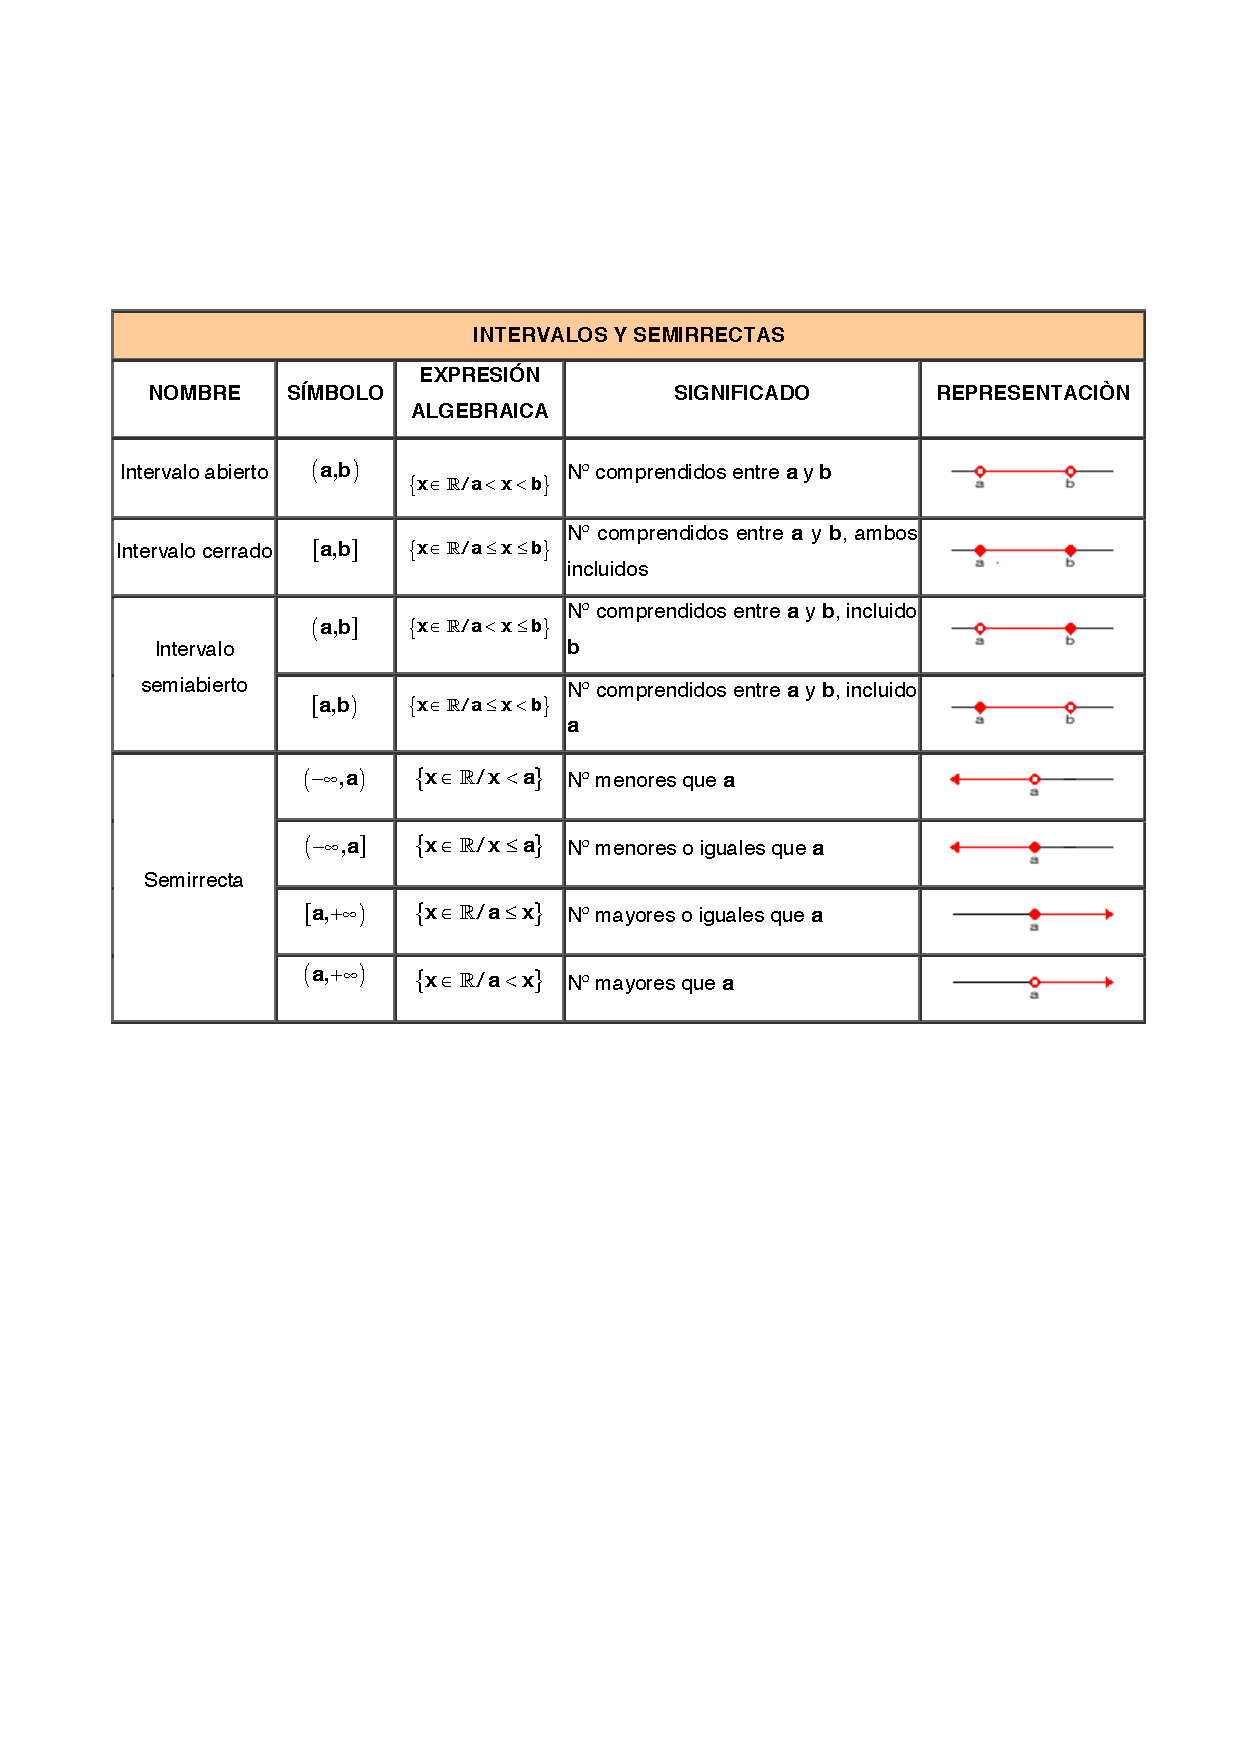
\includegraphics[width=\textwidth]{img-sol/p15-extra}
}

\newcommand{\pagexxix}{
	\heading{Exemples de resolució pel mètode de Gauss}
	
	\subsection*{Sistema Compatible determinat}
	
	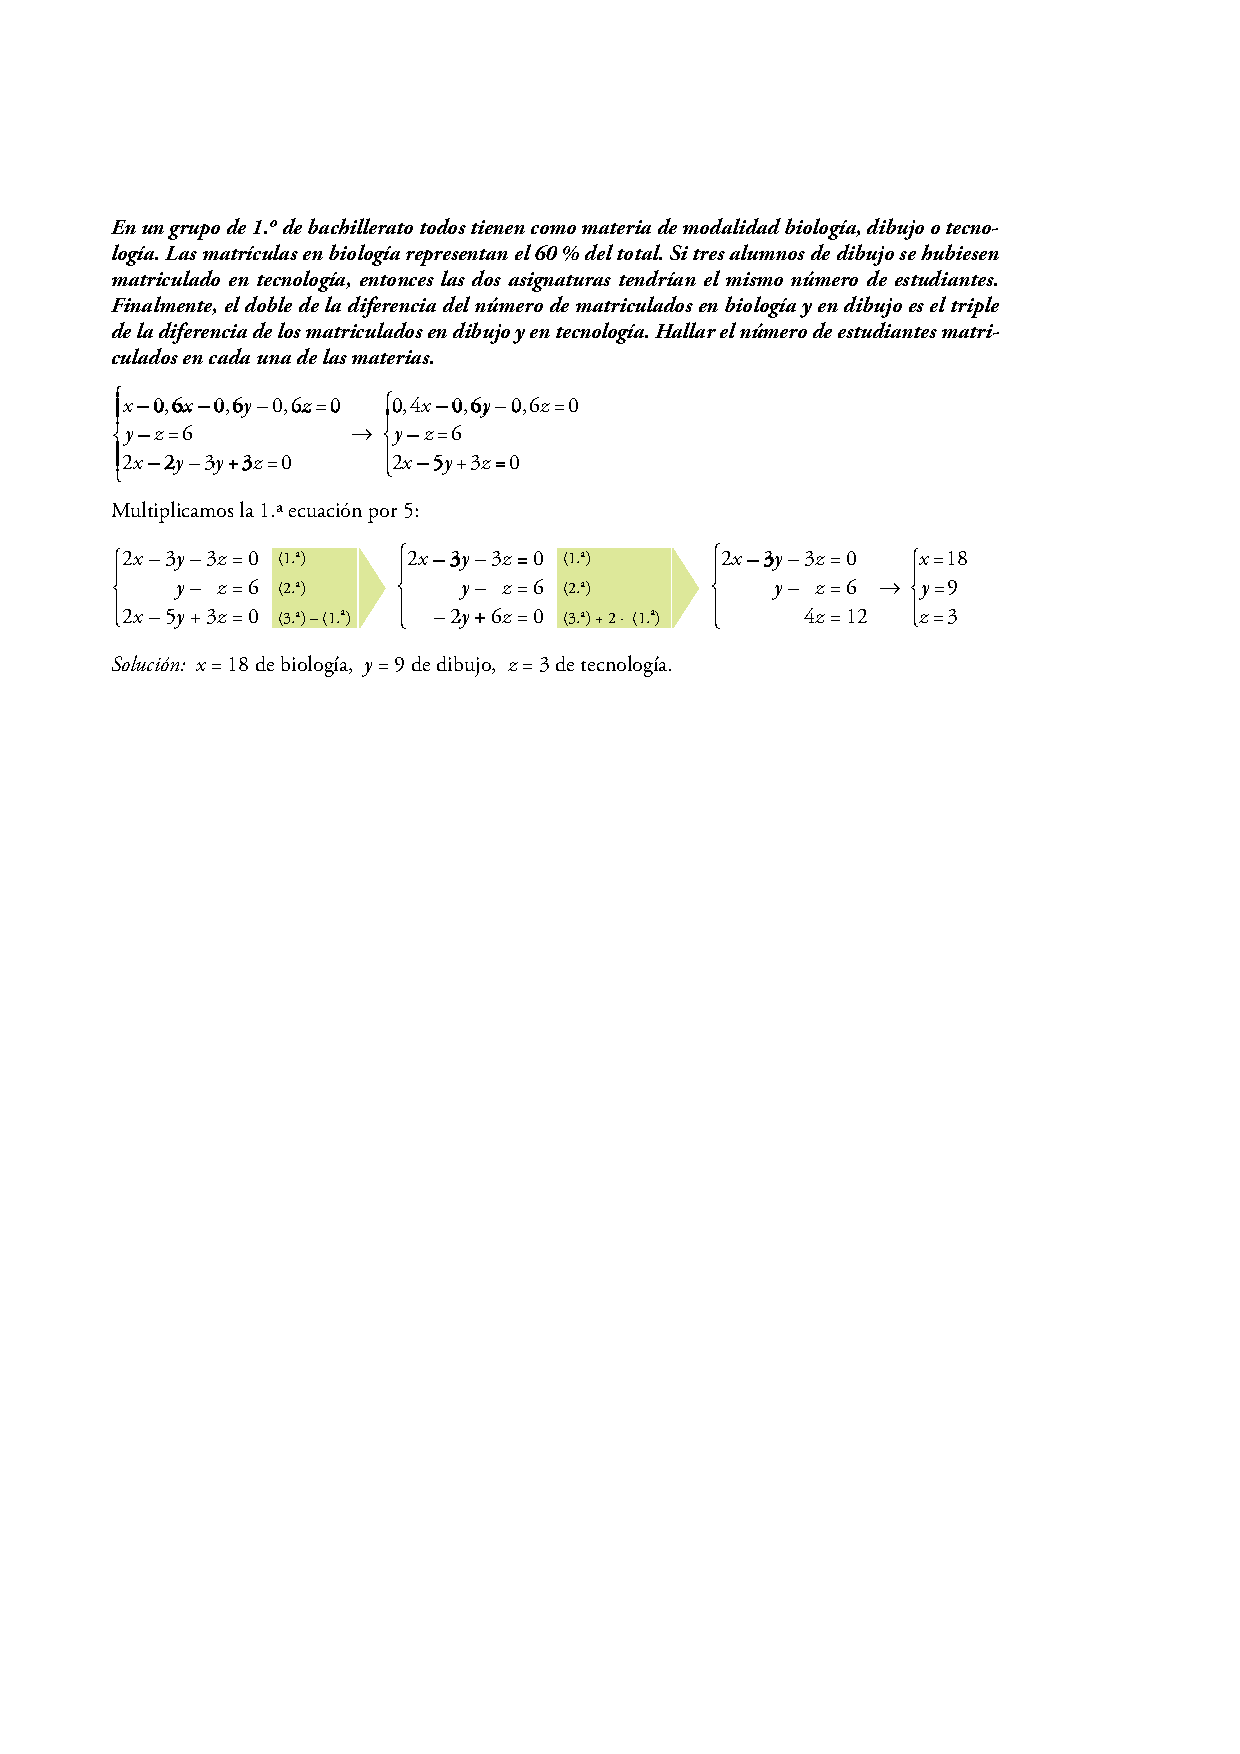
\includegraphics[width=\textwidth]{img-sol/p29-extra1}
	
	\hrule
	
	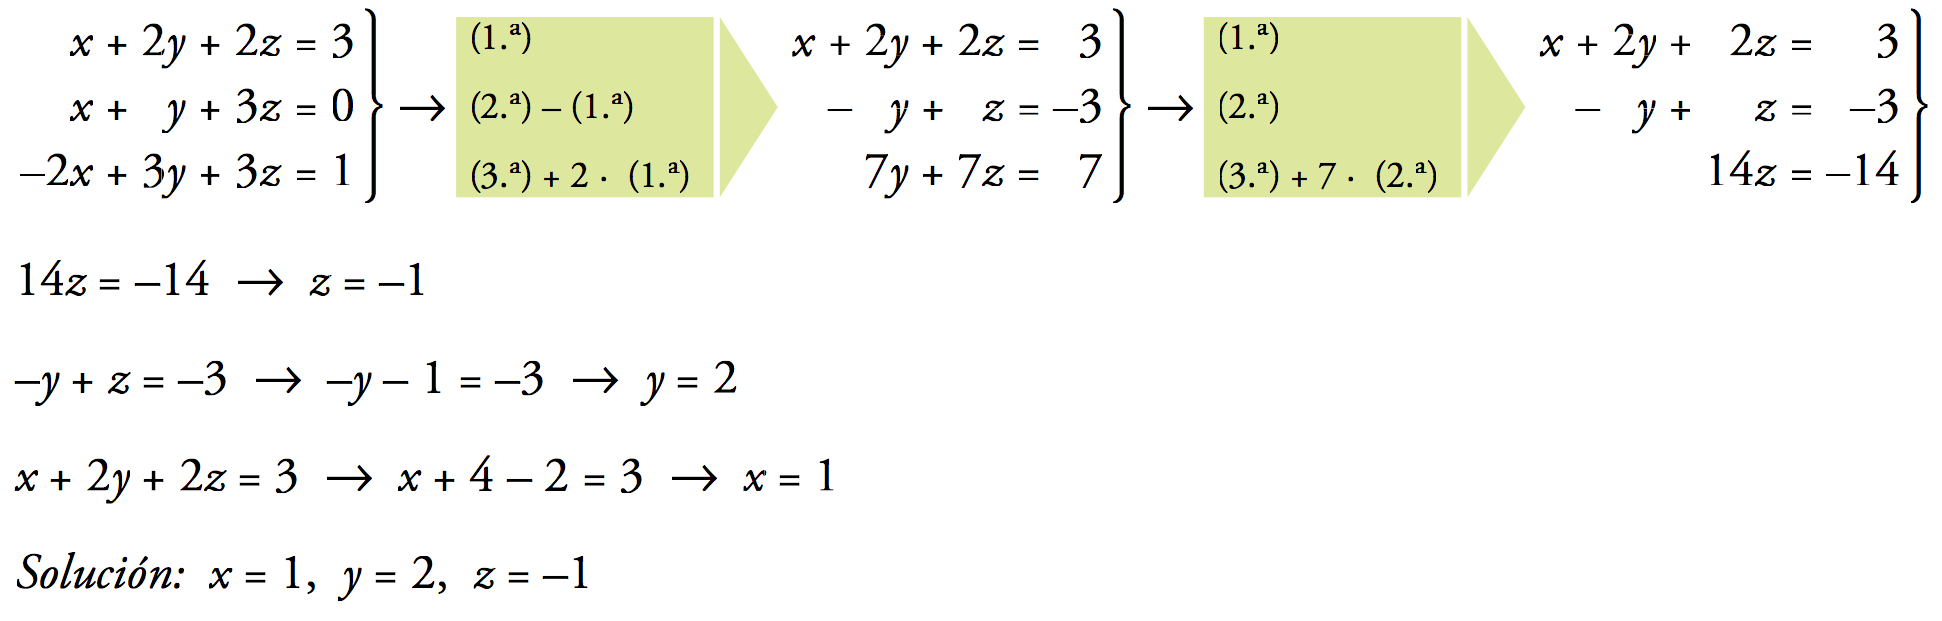
\includegraphics[width=\textwidth]{img-sol/p29-extra2}

	\subsection*{Sistema Compatible indeterminat}
	
	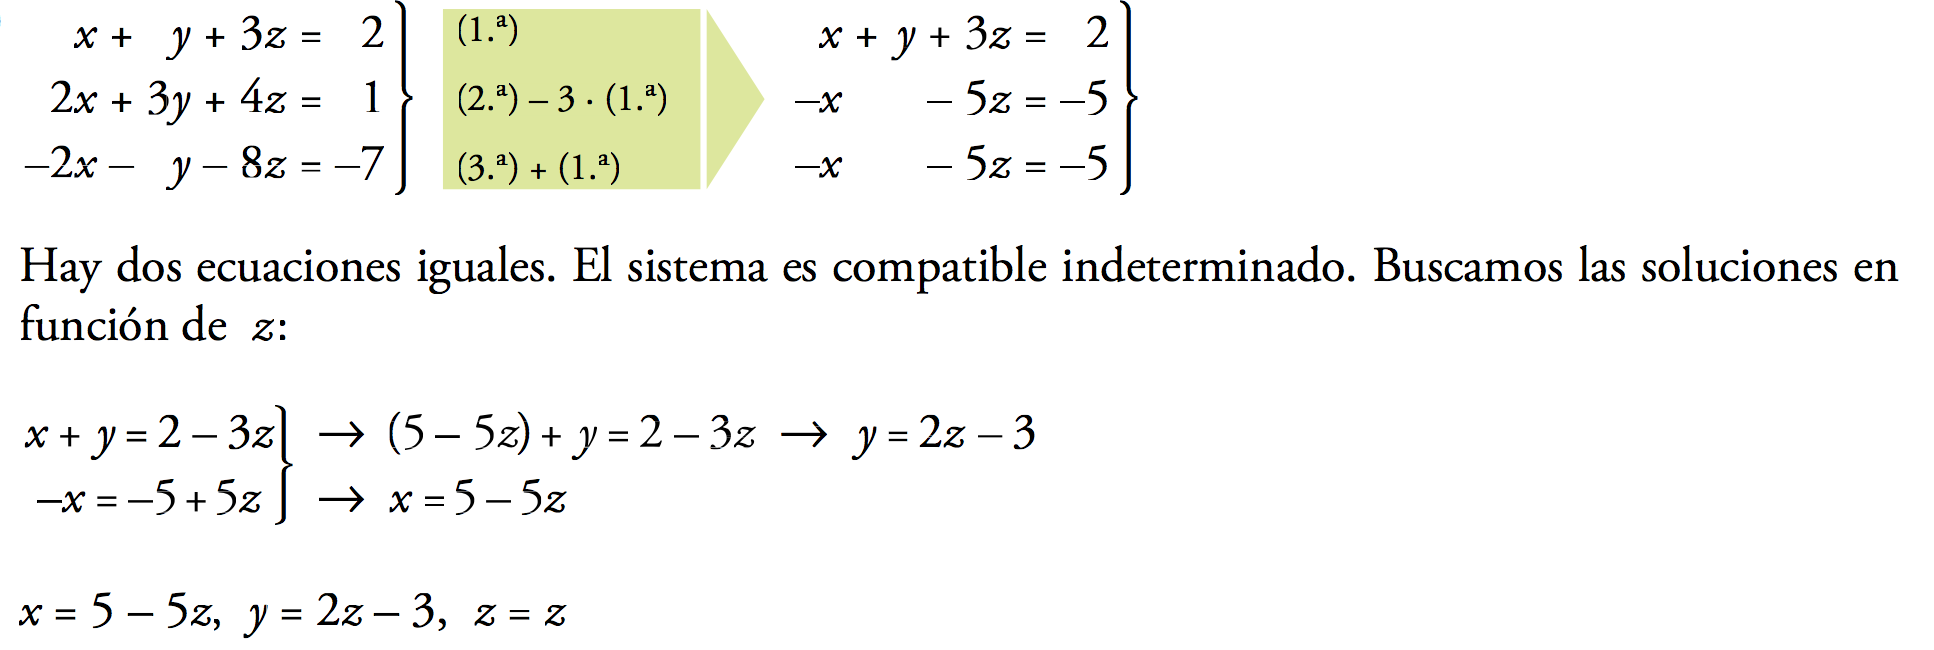
\includegraphics[width=\textwidth]{img-sol/p29-extra3}
}

\newcommand{\pagexxx}{
	\heading{Raons d'angles majors que 90$^\circ$}
 
	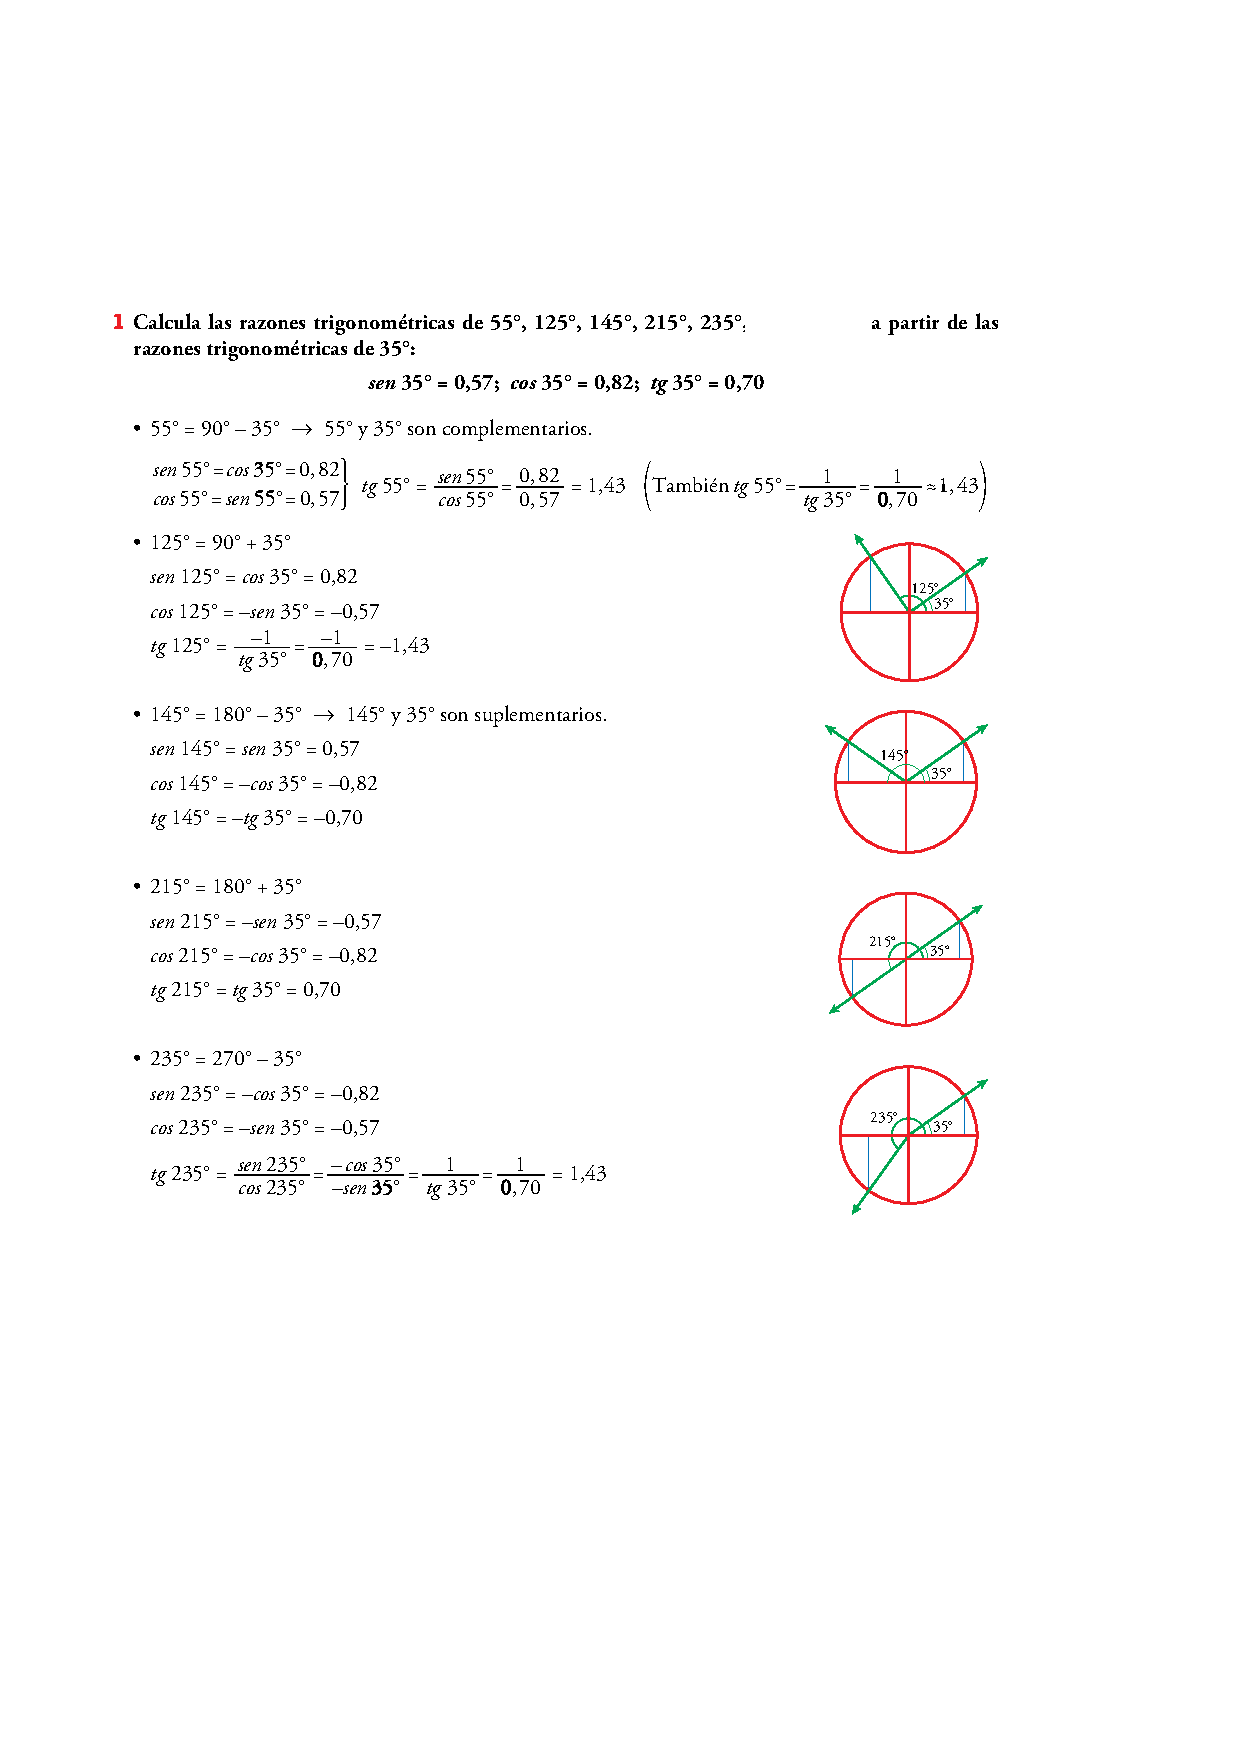
\includegraphics[width=\textwidth]{img-sol/p30-extra1}	
}


\newcommand{\pagexlvii}{
	\heading{Representació dels nombres complexos}
\begin{center}
	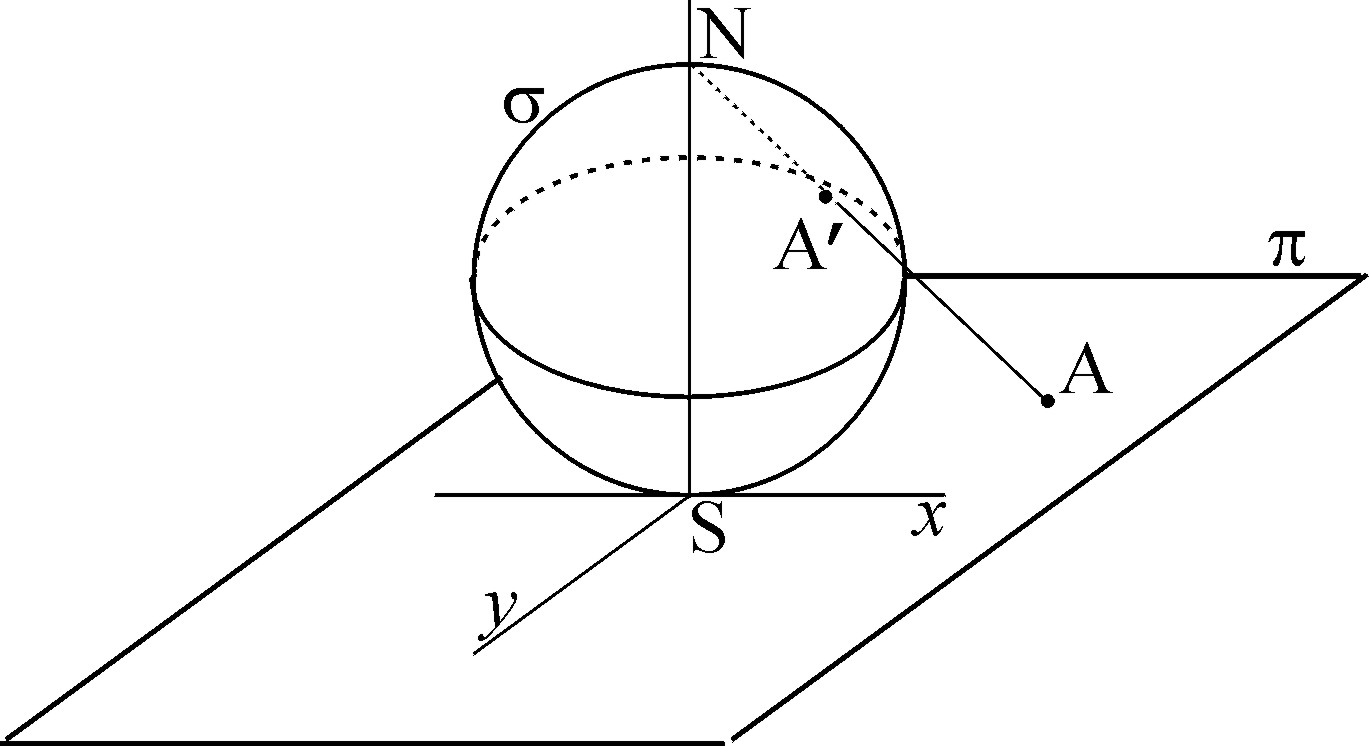
\includegraphics[width=0.5\textwidth]{img-sol/p47-extra1}
\end{center}

\vso 

\heading{Objectius del tema:}

\vspace{0.25cm}
{
	\fontsize{10.5}{12.8}\selectfont
	2. Conèixer els nombres complexos com a extensió dels nombres reals, utilitzant-los per obtenir solucions d’algunes equacions algebraiques.
	
	2.1. Valora els nombres complexos com a ampliació del concepte de nombre real i els utilitza per obtenir la solució d’equacions de segon grau amb coeficients reals sense solució real.
	
	2.2. Opera amb nombres complexos, i els representa gràficament, i utilitza la fórmula de Moivre en el cas de les potències
}

%%%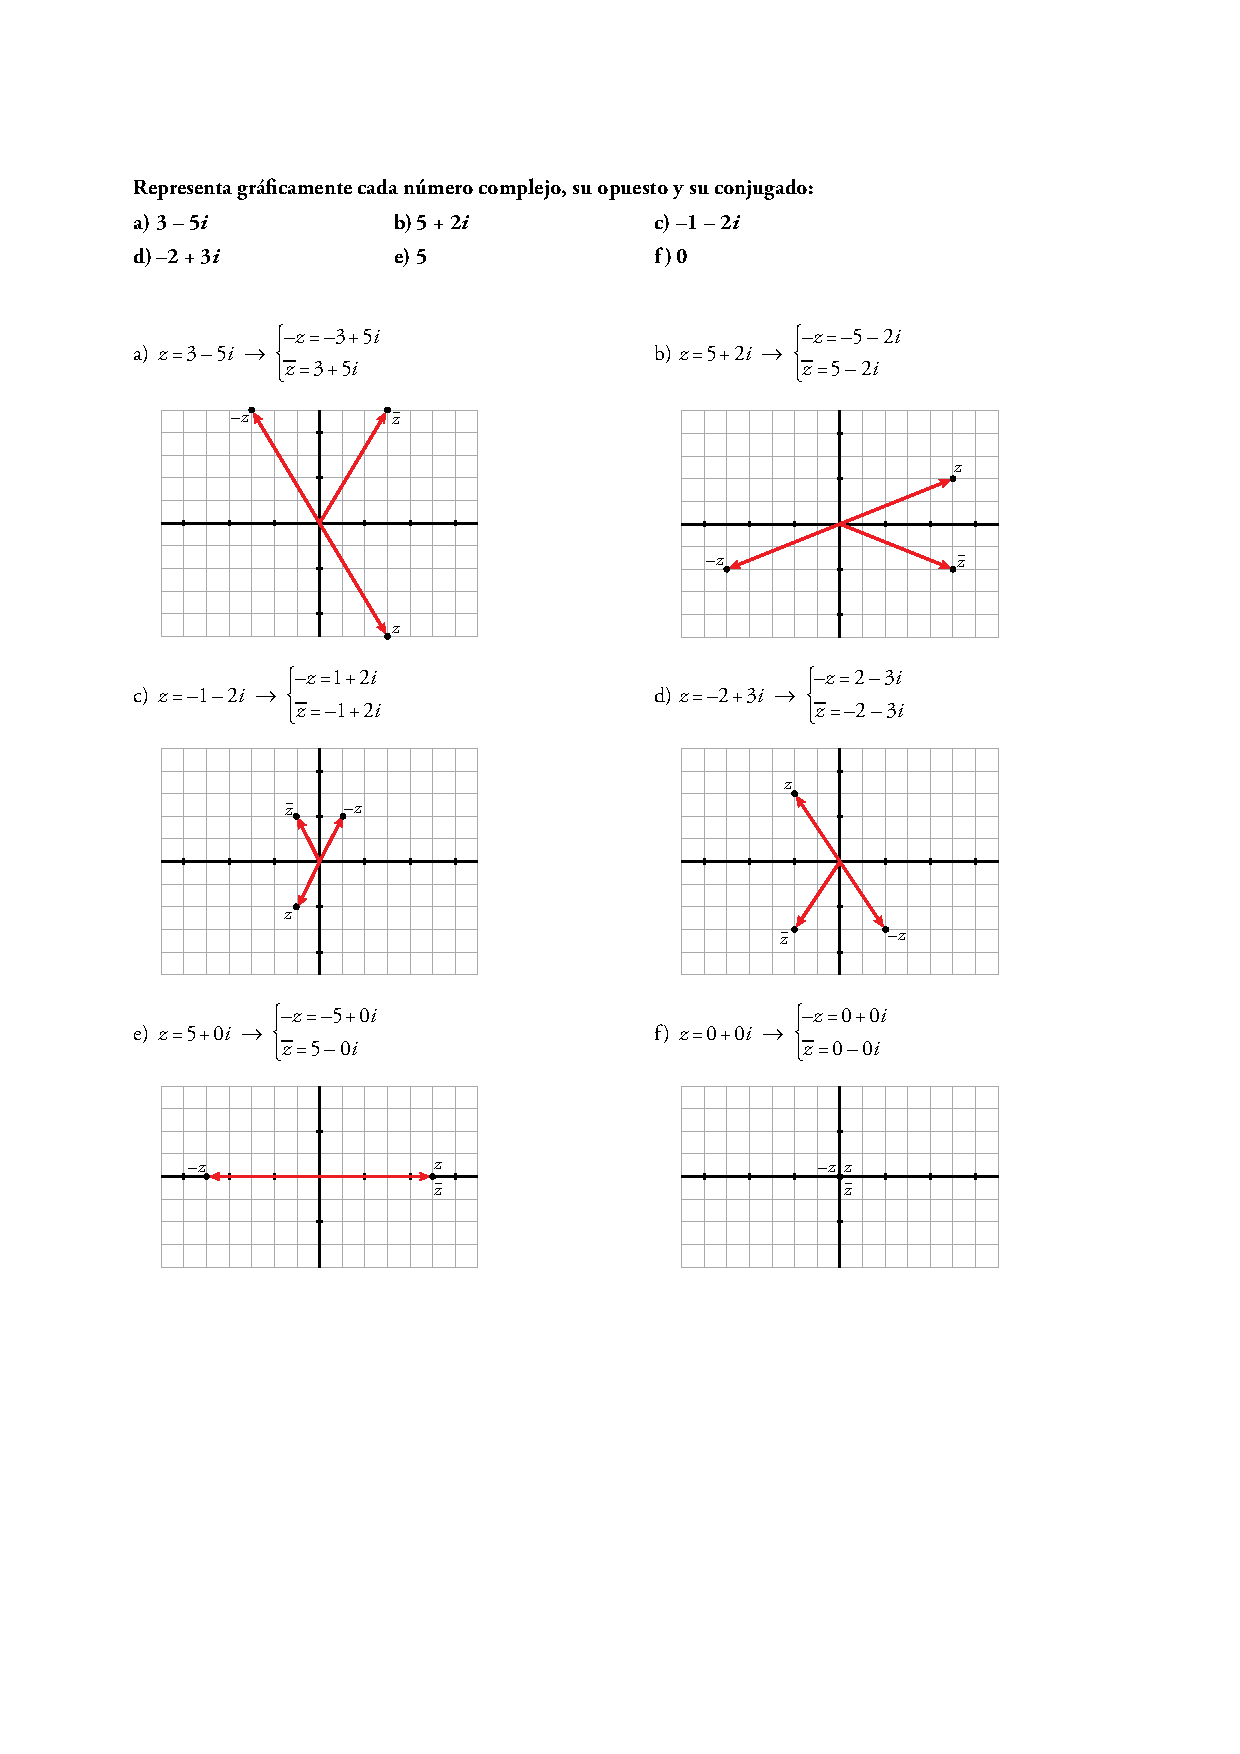
\includegraphics[width=\textwidth]{img-sol/p47-extra2}
}

\newcommand{\pagelxxii}{
\heading{Concepte de límit}

\subsection*{A partir d'una gràfica}
\begin{center}
	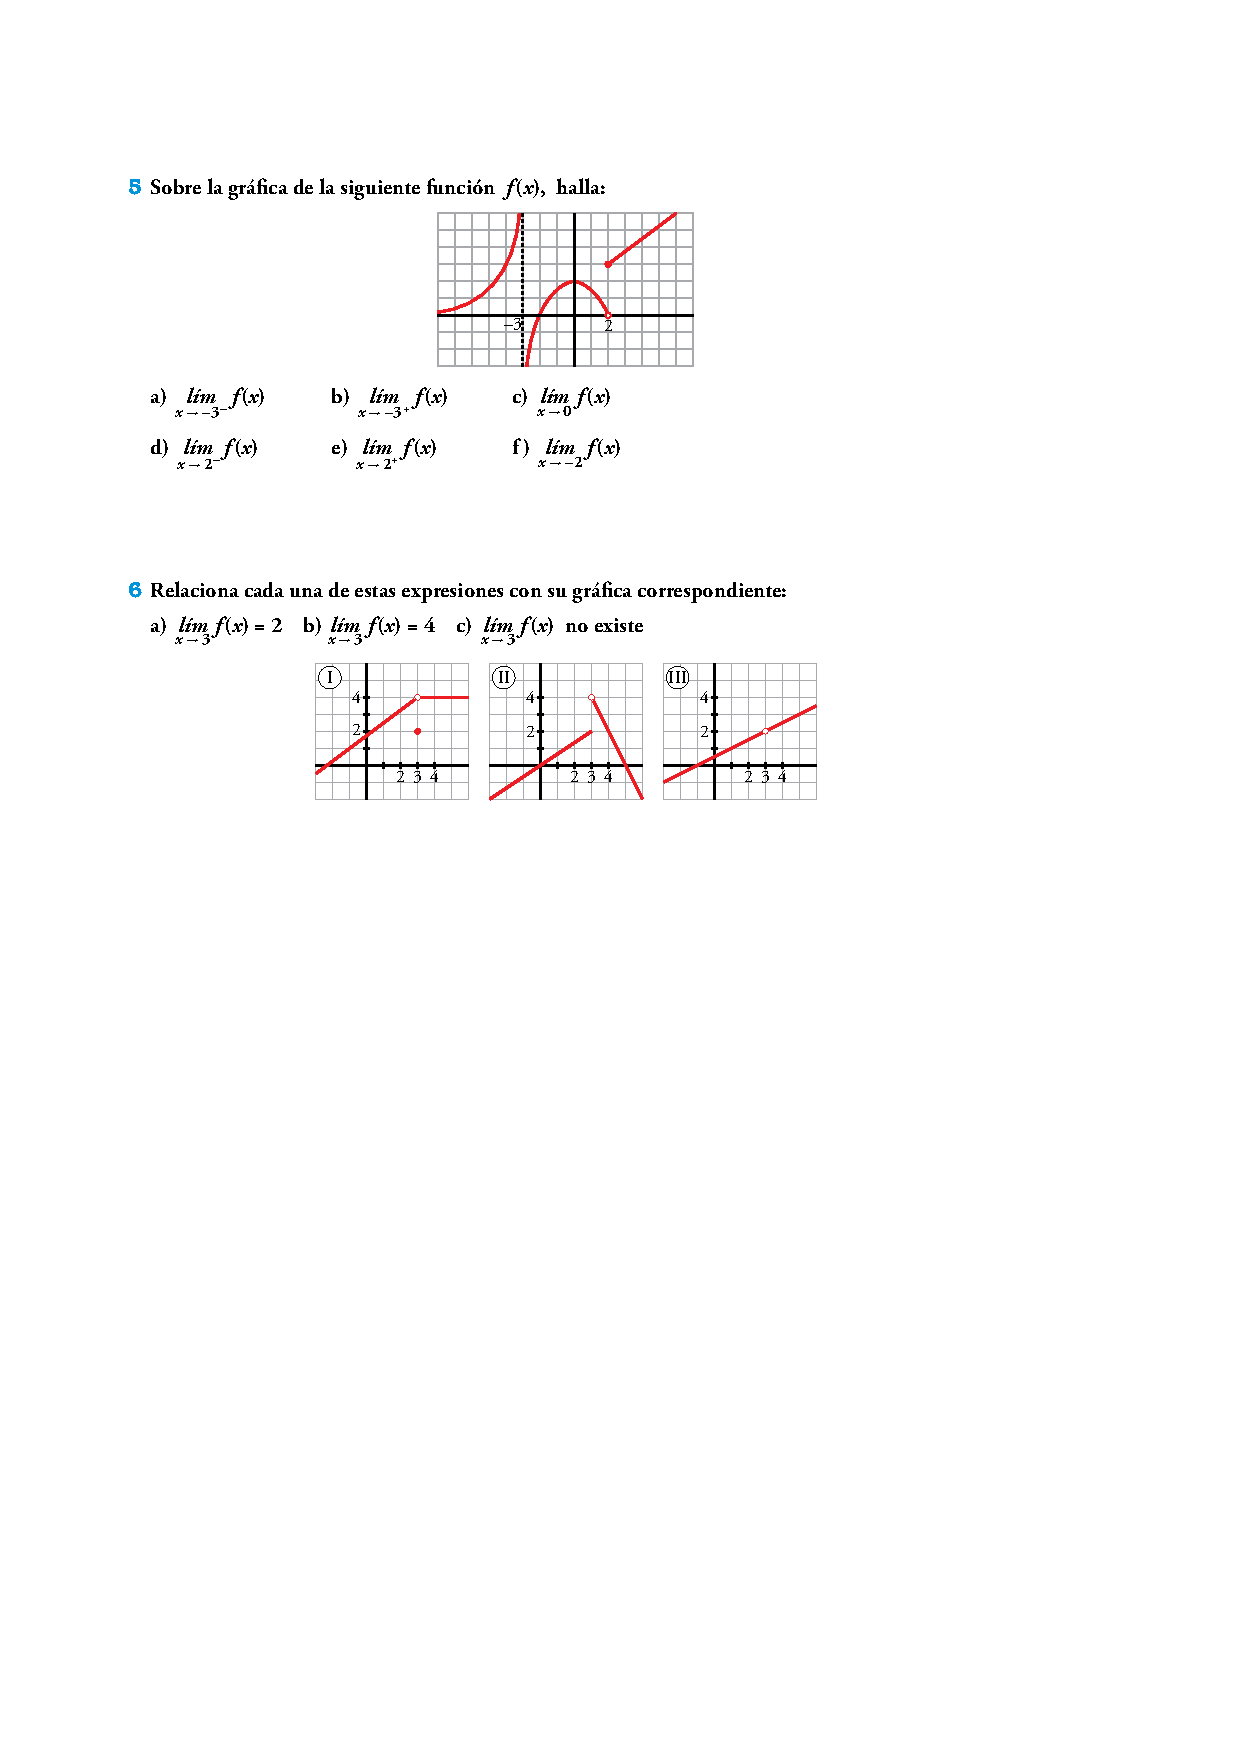
\includegraphics[width=\textwidth]{img-sol/p72-extra1}
\end{center}


\subsection*{A partir d'una taula de valors}

\begin{multicols}{2}
\begin{center}
	\[ f(x)= \dfrac{\sqrt{x}-1}{x^2-1} \]
 \begin{tabular}{|c|c|}\hline
 	$x$ & $y$ \\\hline
 	0.9 & 0.270088\\\hline
 	0.99 & 0.251888\\\hline
 	0.999 & 0.2501876\\\hline
 	0.9999 & 0.2500187\\\hline
 \end{tabular}
\[ \limx{1^-} \dfrac{\sqrt{x}-1}{x^2-1}=0.25=\dfrac{1}{4}\]
\columnbreak
	\[ f(x)= \dfrac{2x+1}{\sqrt{x}} \]
\begin{tabular}{|c|c|}\hline
	$x$ & $y$ \\\hline
	10 & 6.641 \\\hline
	1000 & 63.277 \\\hline
	1000000 & 2000.001 \\\hline
	100000000 & 20000.001 \\\hline
\end{tabular}
\[ \limx{+\infty} \dfrac{2x+1}{\sqrt{x}}=+\infty\]

\end{center}
\end{multicols}
}

\newcommand{\pagelviii}{
	\vspace*{\fill}
	\begin{center}
		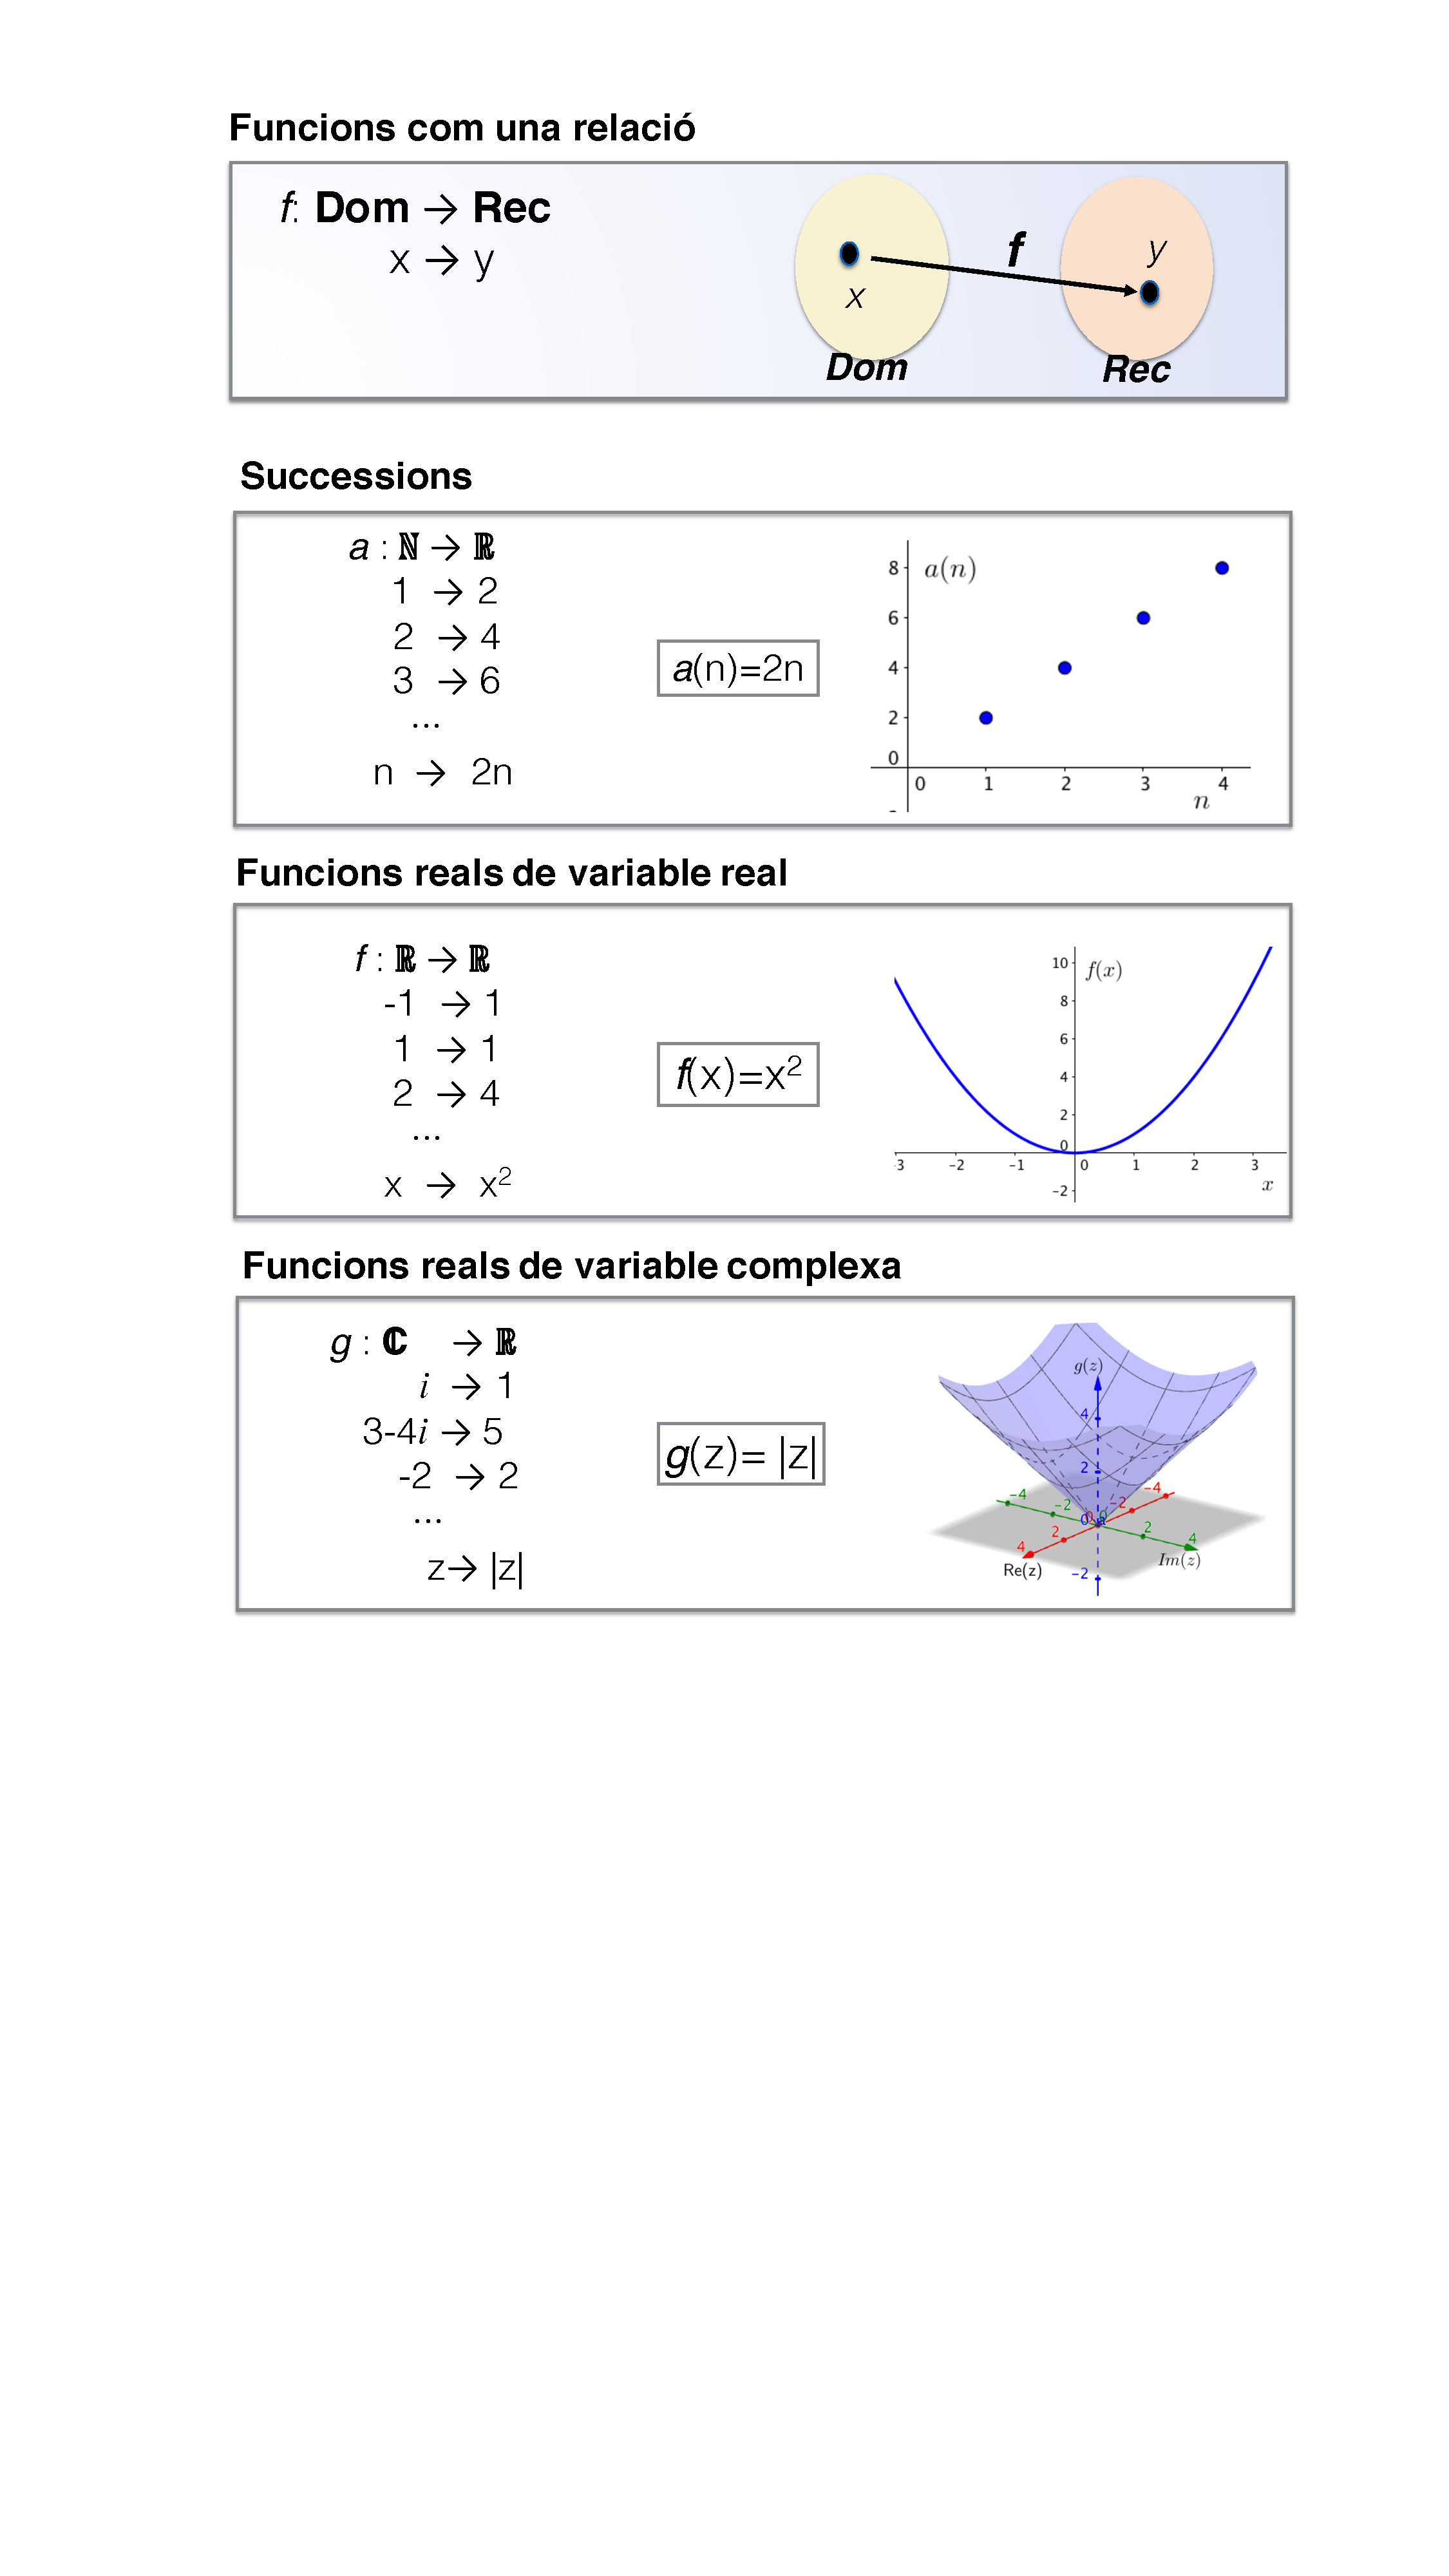
\includegraphics[width=0.8\textwidth]{img-sol/p58-extra1}
	\end{center}
	\vspace*{\fill}
}
 

\newcommand{\pagelxxv}{
\heading{Exemple càlcul de límits amb radicals}

\vso

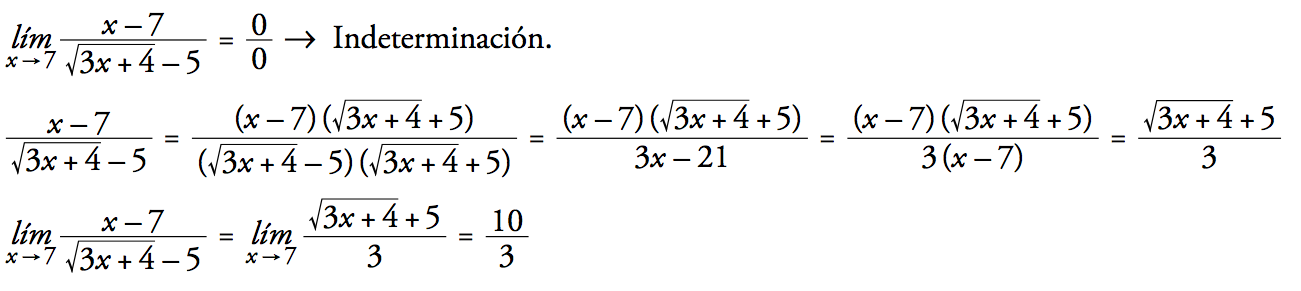
\includegraphics[width=\textwidth]{img-sol/p75-extra1}

\vso
\hrule
\vso

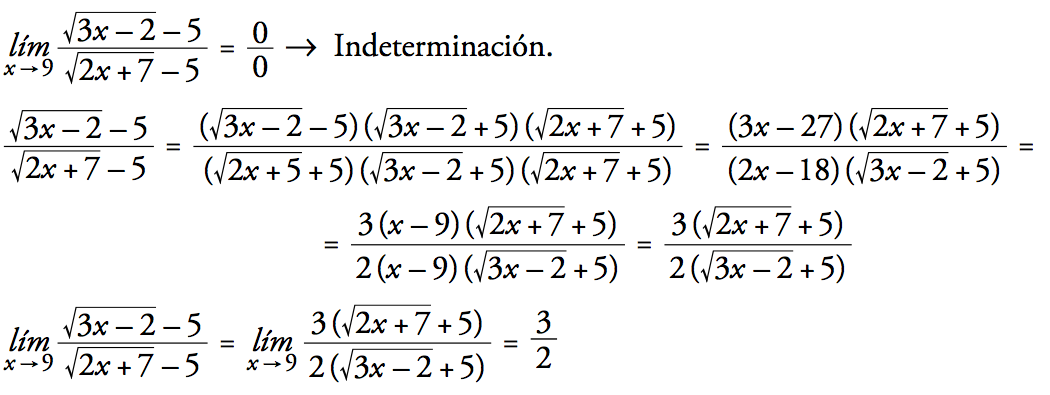
\includegraphics[width=\textwidth]{img-sol/p75-extra2}
}

\newcommand{\pagelxxix}{
\textbf{\large $\bullet$ Gràfics Ex. 14:}

\begin{center}
a) 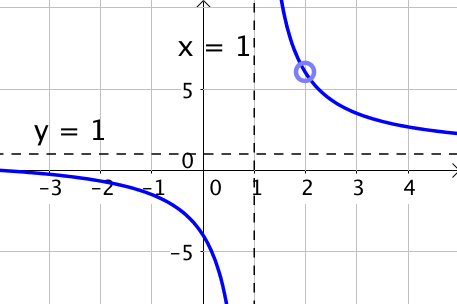
\includegraphics[width=0.38\textwidth]{img-sol/p79-extra-a}
b) 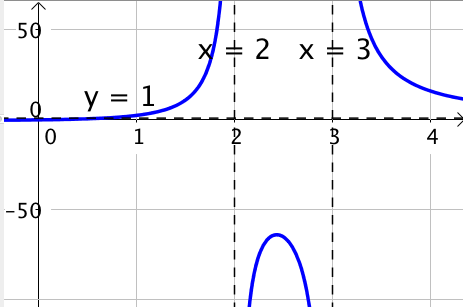
\includegraphics[width=0.38\textwidth]{img-sol/p79-extra-b}

c) 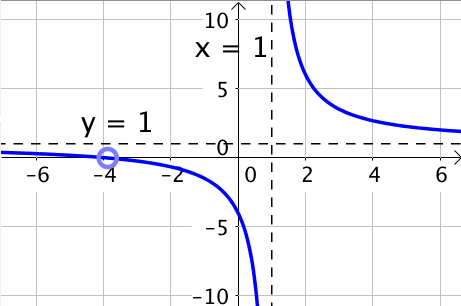
\includegraphics[width=0.38\textwidth]{img-sol/p79-extra-c}
d) 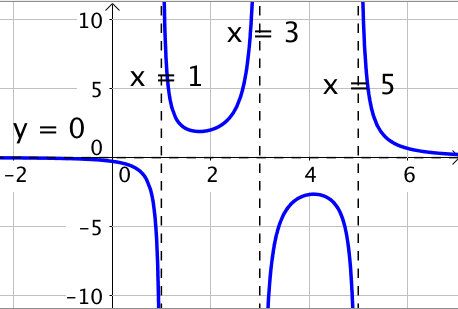
\includegraphics[width=0.38\textwidth]{img-sol/p79-extra-d}
\end{center}
}


\newcommand{\pagelxxx}{
	\textbf{\large $\bullet$ Gràfics Ex. 16:}
	
	\begin{center}
		a) 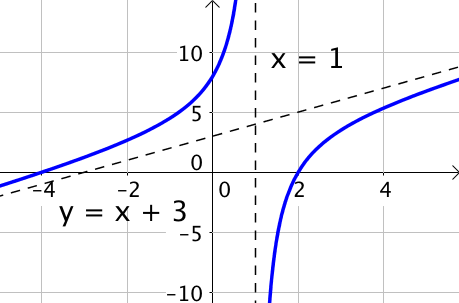
\includegraphics[width=0.38\textwidth]{img-sol/p80-extra-a}
		b) 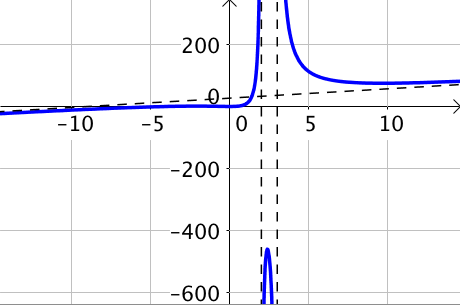
\includegraphics[width=0.38\textwidth]{img-sol/p80-extra-b}
		
		c) 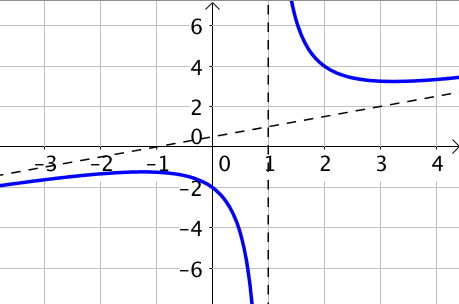
\includegraphics[width=0.38\textwidth]{img-sol/p80-extra-c}
		d) 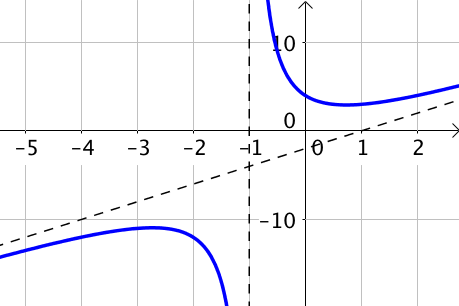
\includegraphics[width=0.38\textwidth]{img-sol/p80-extra-d}
	\end{center}
}


\newcommand{\pagelxxxi}{
	\textbf{\large $\bullet$ Gràfics Ex. 19:}
	
	\begin{center}
		a) 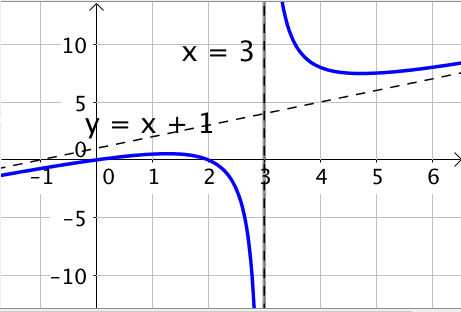
\includegraphics[width=0.35\textwidth]{img-sol/p81-extra-a}
		b) 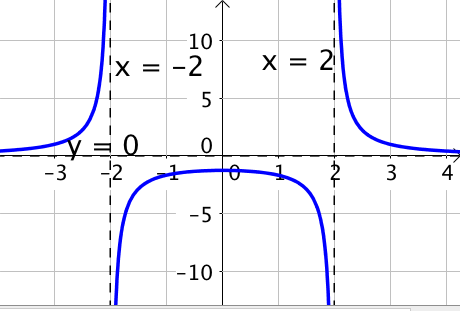
\includegraphics[width=0.35\textwidth]{img-sol/p81-extra-b}
		
		c) 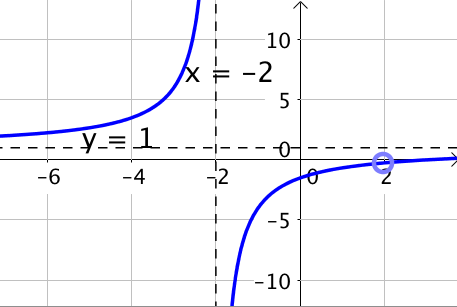
\includegraphics[width=0.35\textwidth]{img-sol/p81-extra-c}
		d) 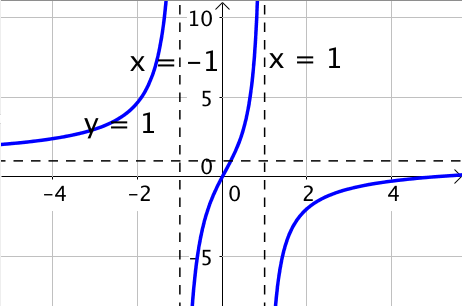
\includegraphics[width=0.35\textwidth]{img-sol/p81-extra-d}
		
		e) 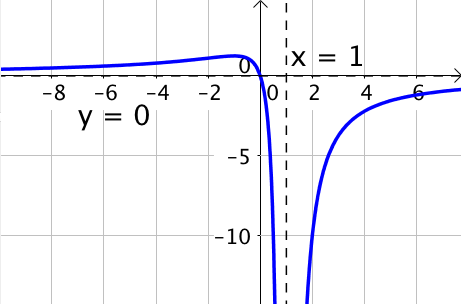
\includegraphics[width=0.35\textwidth]{img-sol/p81-extra-e}
		f) 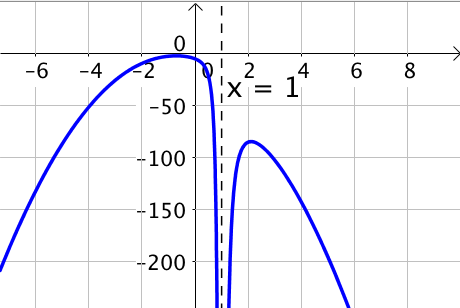
\includegraphics[width=0.35\textwidth]{img-sol/p81-extra-f}
		
		g) 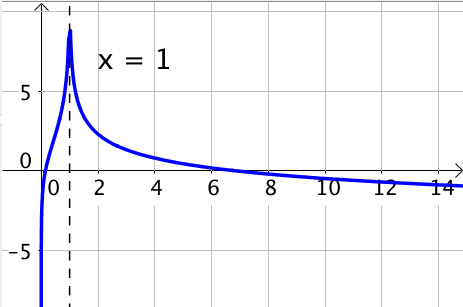
\includegraphics[width=0.35\textwidth]{img-sol/p81-extra-g}
		h) 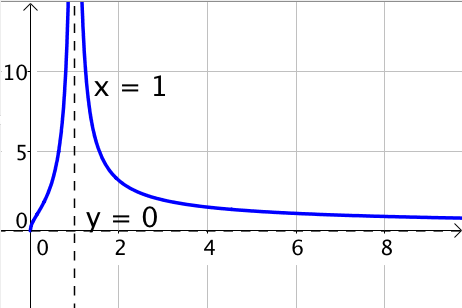
\includegraphics[width=0.35\textwidth]{img-sol/p81-extra-h}
	\end{center}
}

\newcommand{\pagecii}{
\newpage

\heading{Exemples de problemes d'optimització}

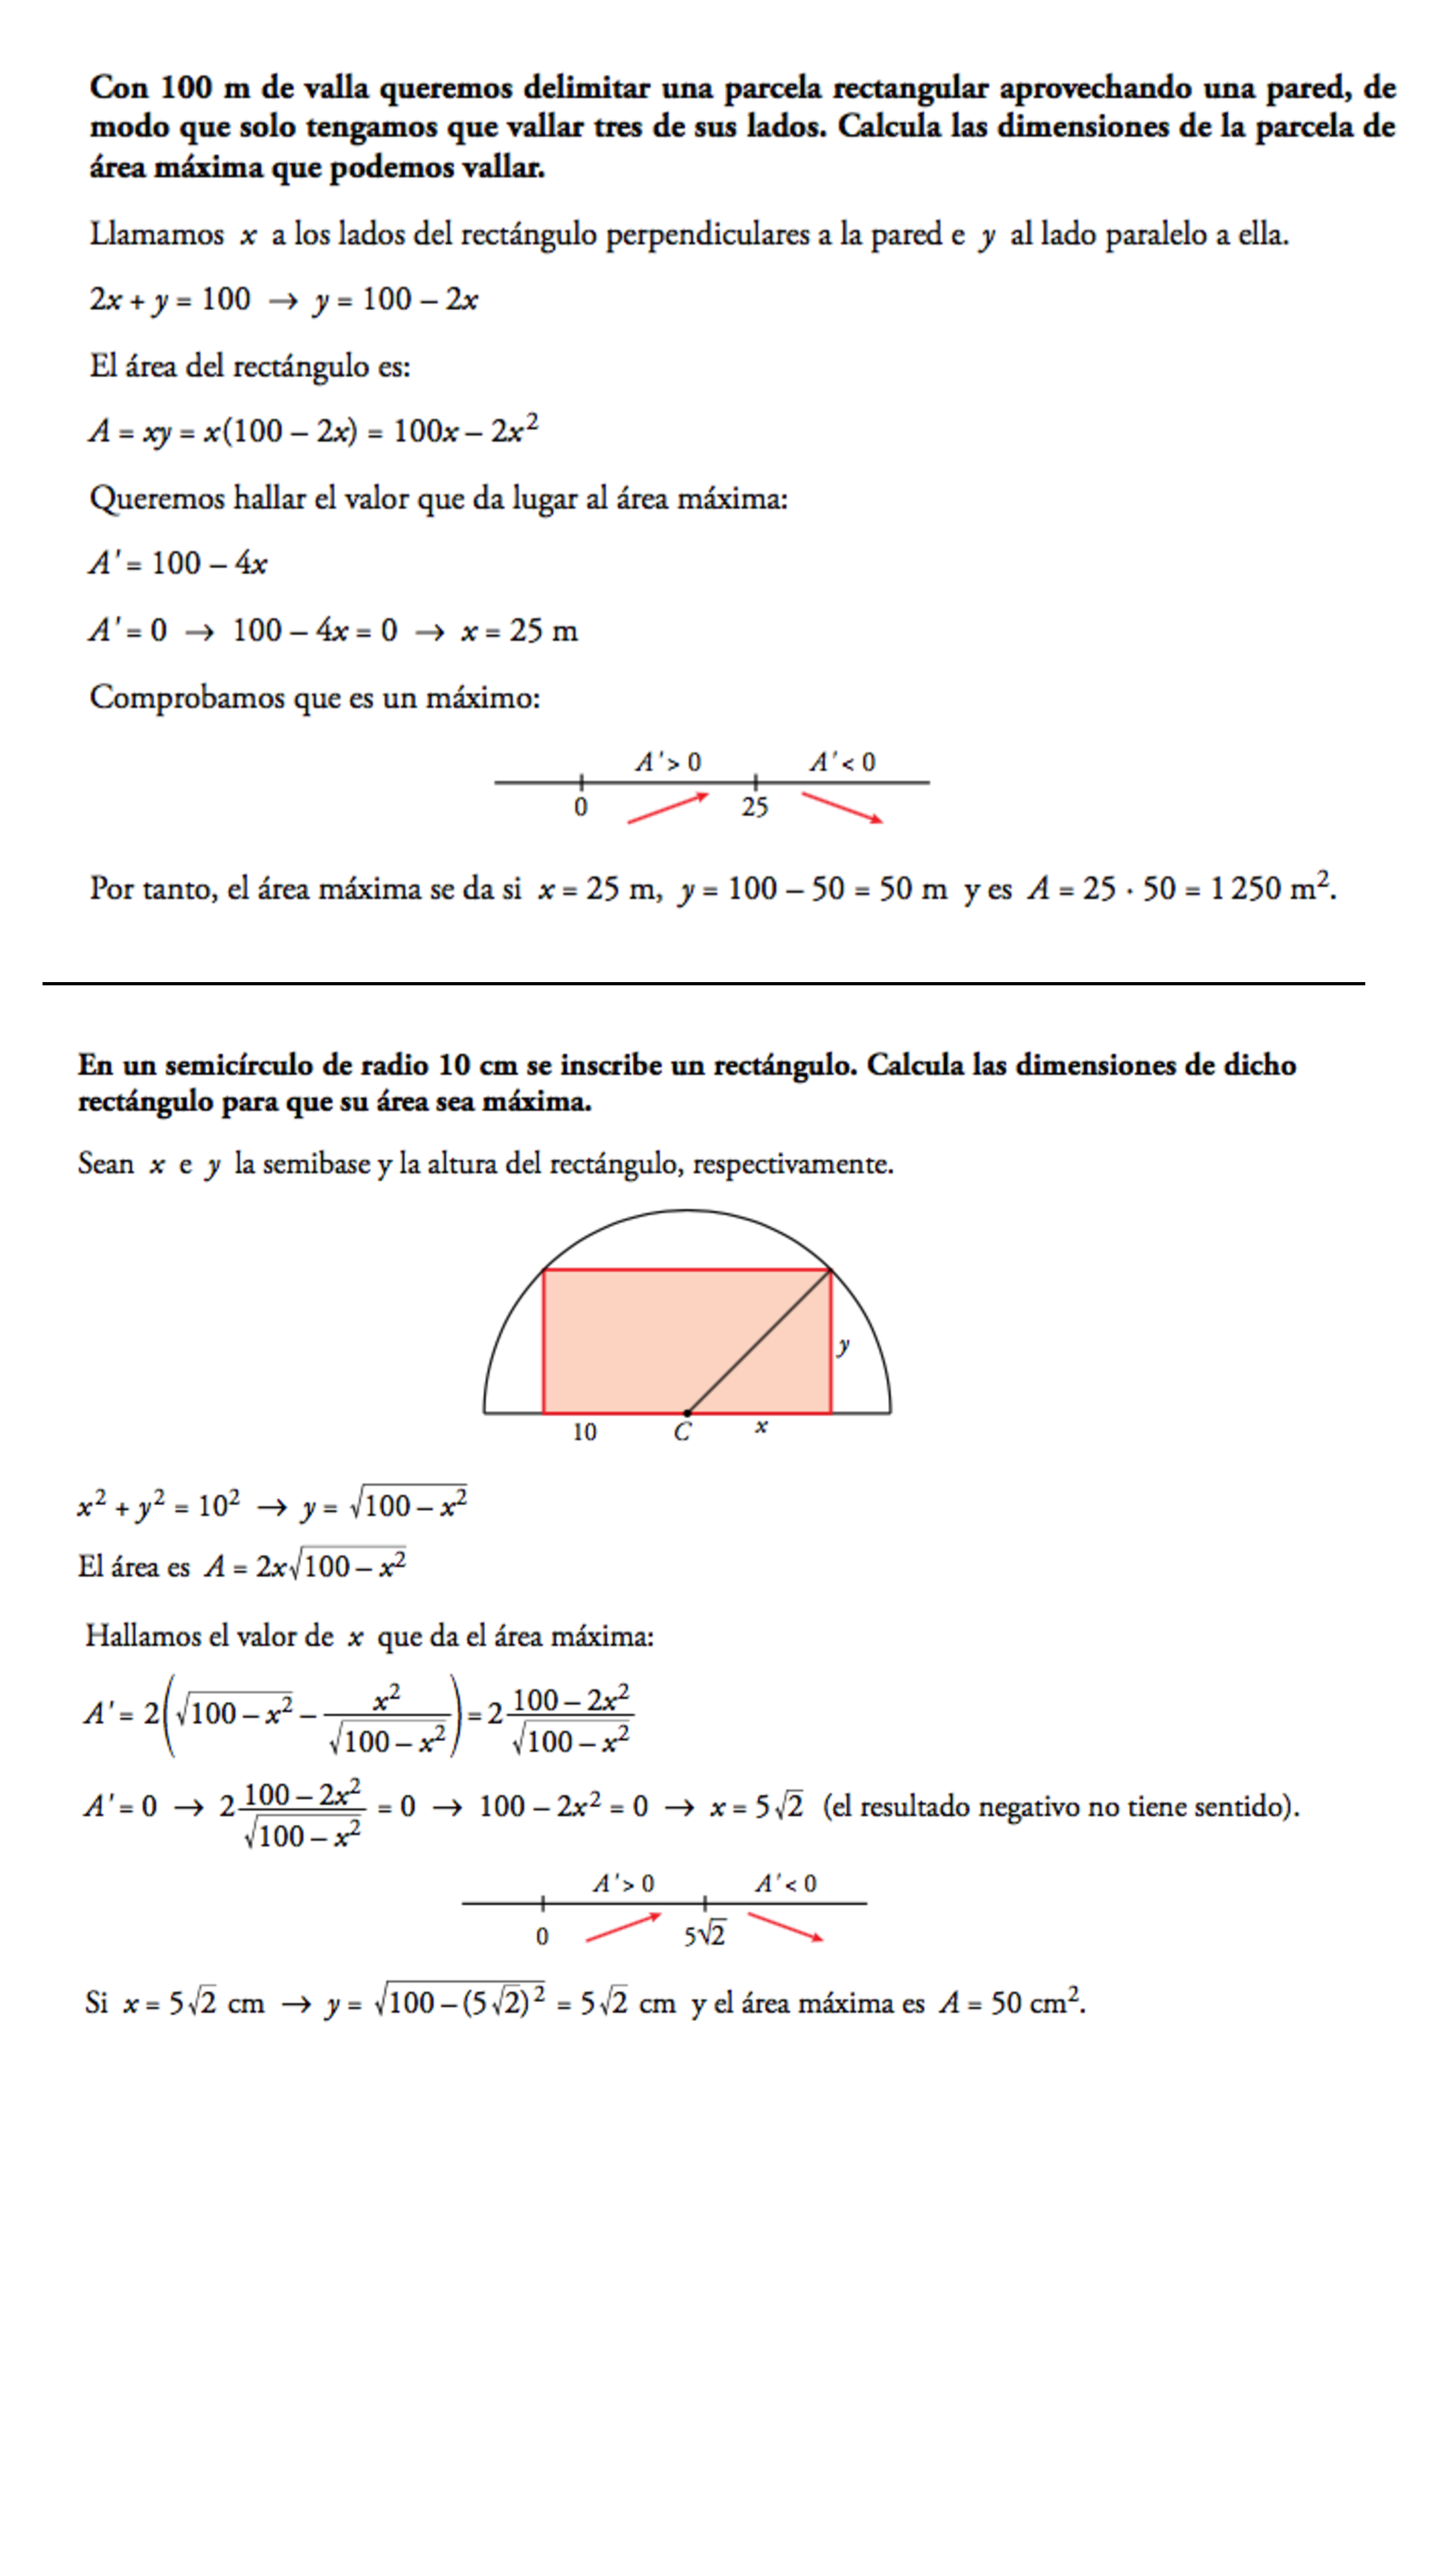
\includegraphics[width=0.95\textwidth]{img-sol/p99-extra}
}


\newcommand{\pagecx}{
\heading{Operacions amb vectors gràficament}

\vso
\begin{center}
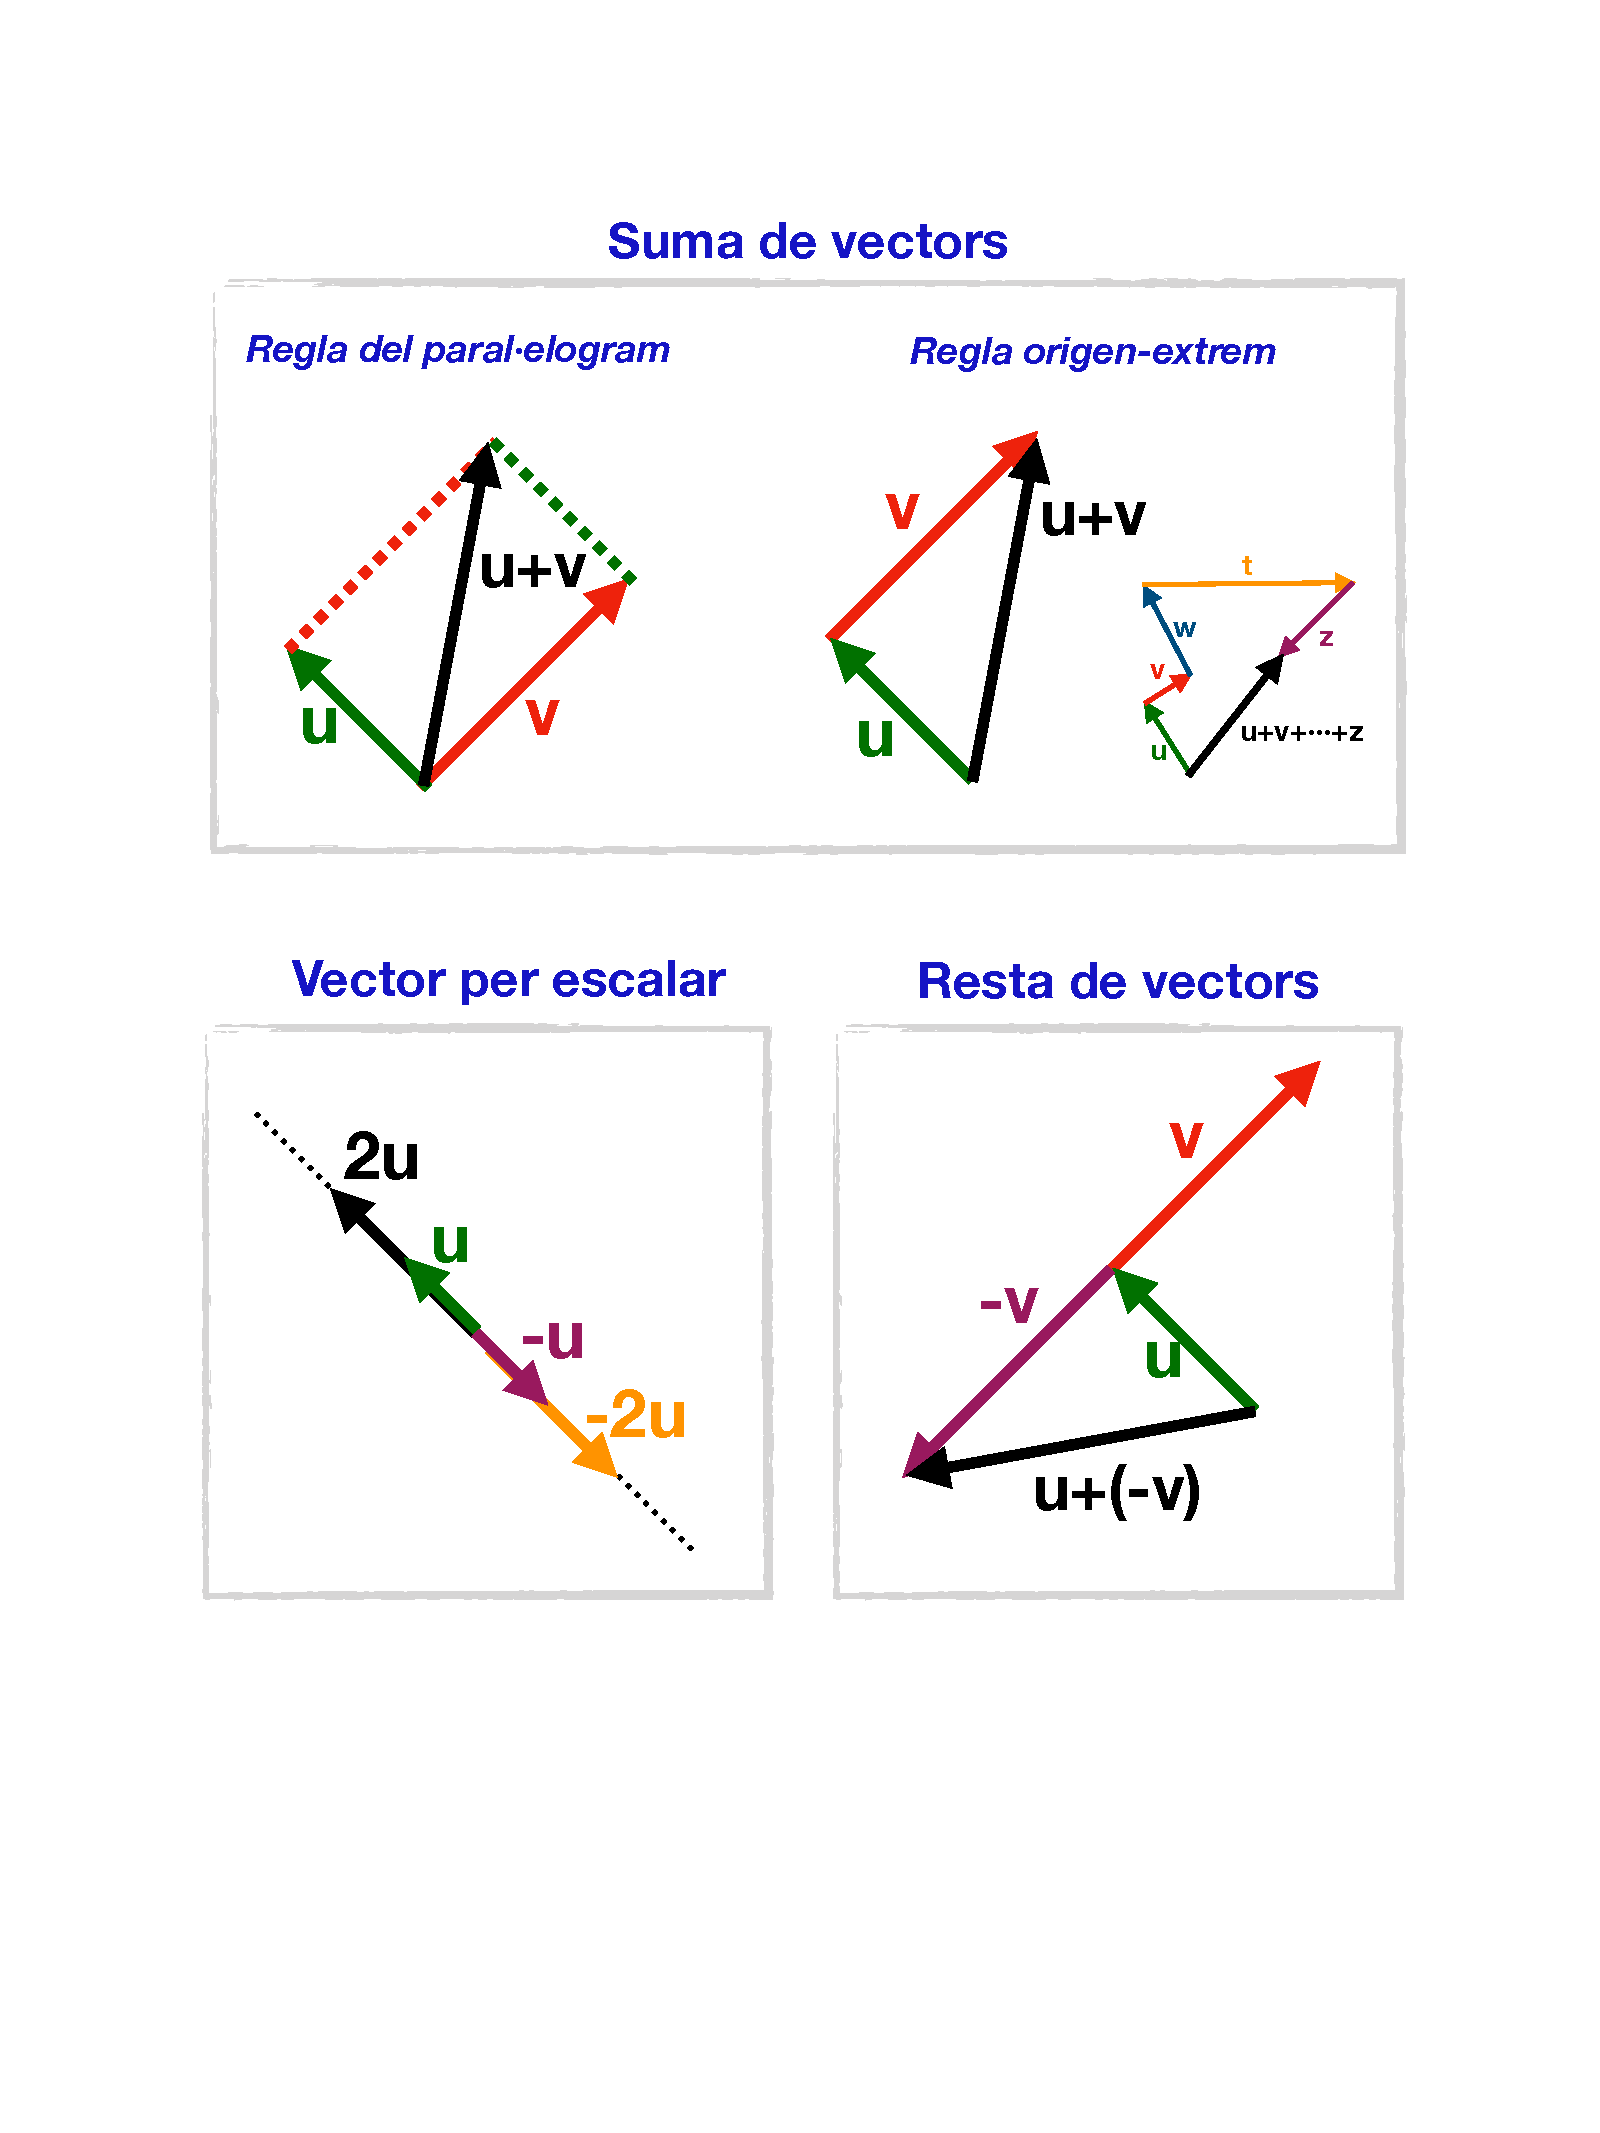
\includegraphics[width=0.75\textwidth]{img-sol/p110-extra}
\end{center}
\vso

\heading{Objectius del tema:}

\vspace{0.25cm}
{
	\fontsize{10.5}{12.8}\selectfont
	 3. Fer servir l’operació del producte escalar i les seves conseqüències. Entendre els conceptes de base ortogonal i ortonormal. Distingir i manejar-se amb precisió en el pla euclidià i en el pla mètric, utilitzant en ambdós casos les seves eines i propietats.
	 
3.1. Empra amb assiduïtat les conseqüències de la definició de producte escalar per normalitzar vectors, calcular el cosinus d’un angle, estudiar l’ortogonalitat de dos vectors o la projecció d’un vector sobre un altre.

3.2. Calcula l’expressió analítica del producte escalar, del mòdul i del cosinus de l’angle.

}
}

\newcommand{\pagecxxiv}{
	\heading{Demostració fórmula distància punt -- recta}
	
	\begin{center}
		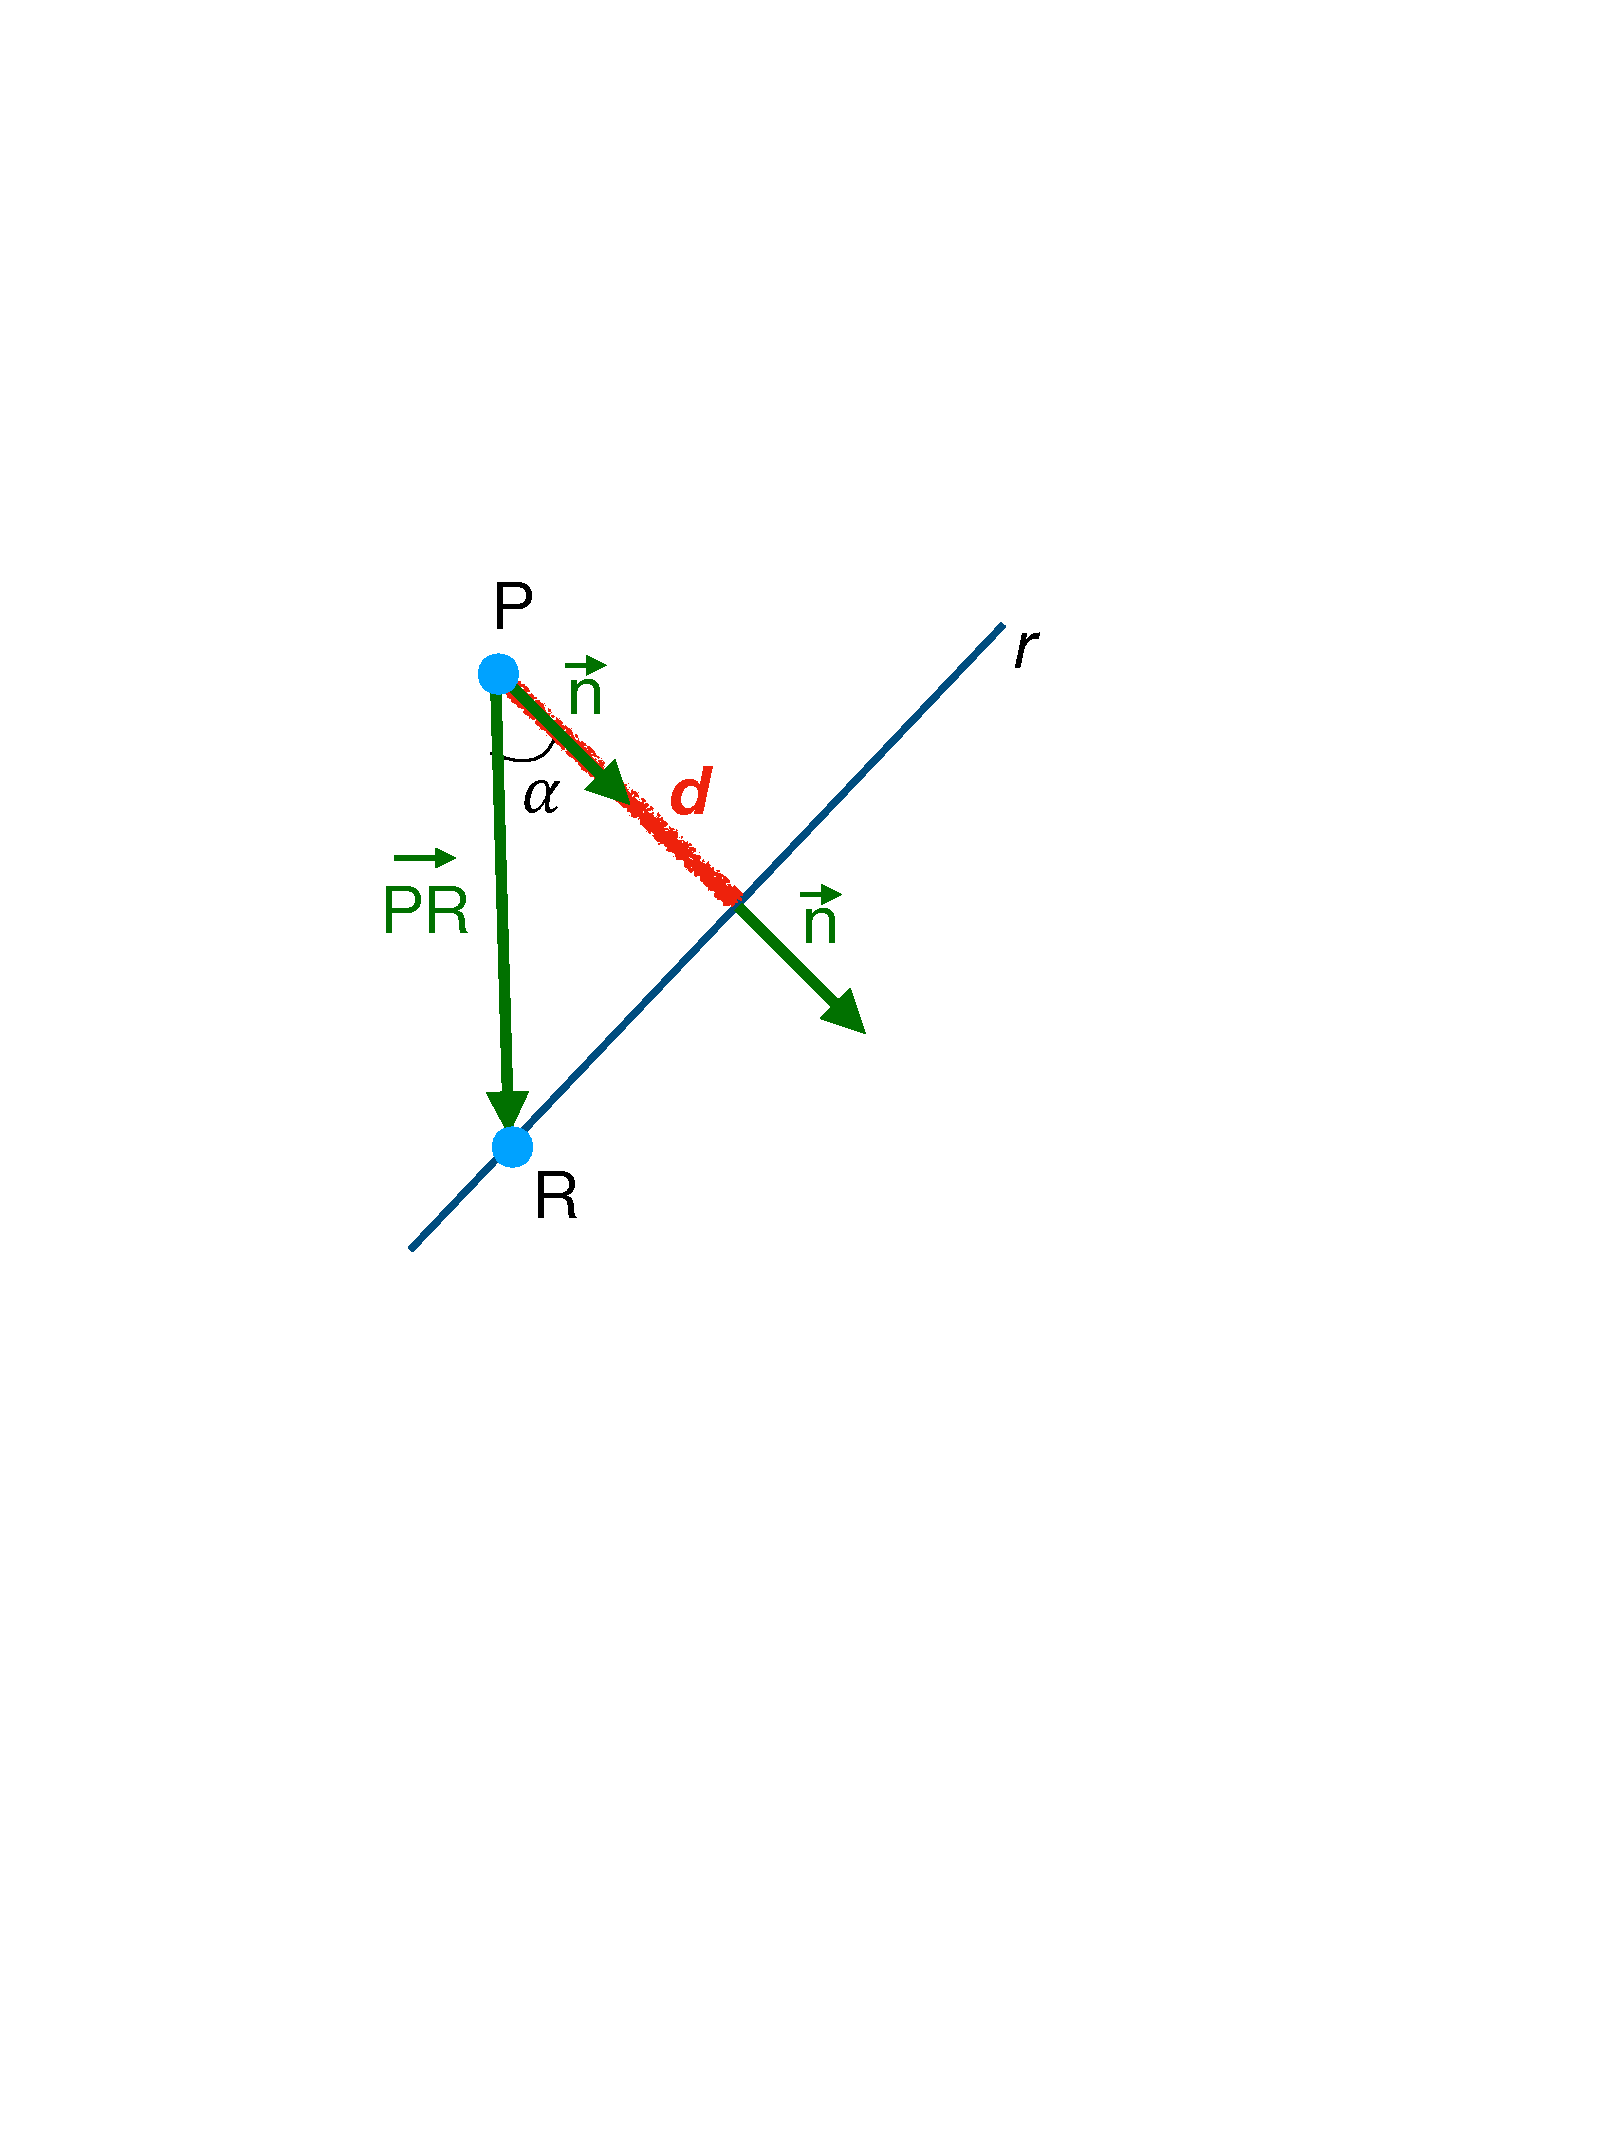
\includegraphics[width=0.4\textwidth]{img-sol/dem-dist-pr}
	\end{center}

	{
	\large
	
	Suposem que la recta $r$ vengui donada en forma general $Ax+By+C=0$. Recordem que el vector normal a la recta és $\vec n = (A,B)$.
	
	Si $R$ és un punt qualsevol de la recta i $\vec n$ és el seu vector normal, observam de l'esquema de la figura que la distància s'obté per trigonometria
	\[
		d = |\overrightarrow{PR}| \cos \alpha
	\]
	
	Per definició de producte escalar:
	\[
		\overrightarrow{PR} \cdot \vec n = |\overrightarrow{PR}|\, |\vec n| \, \cos \alpha
	\]
	
	Si aïllam $\cos \alpha$ i ho reemplaçam en la fórmula anterior, trobam:
	\[
		d = \dfrac{	\overrightarrow{PR} \cdot \vec n}{ |\vec n| } = \dfrac{
		(R_x-P_x, R_y-P_y)\cdot (A,B)}{\sqrt{A^2+B^2}}
	\]
	
	Si desenvolupam $(R_x-P_x, R_y-P_y)\cdot (A,B) = AR_x+B R_y - (AP_x+B P_y)=-C-(A P_x+B P_y)$. Aquí hem utilitzat el fet que el punt $R$ pertany a la recta i, per tant, compleix la seva equació $A R_x+B R_y+C=0$.
	
	Finalment
	
		\[d =  \dfrac{|A P_x+ B P_y +C|}{\sqrt{A^2+B^2}} \]
	
	el valor absolut $|\;|$ és per assegurar que les distàncies surtin positives.
	}
}

%%% Llocs o circumferencia
\newcommand{\pagecxxxi}{

\heading{Mètode de completar quadrats}

Quan tenim una identitat notable és evident que 

\[ x^2 - 2x + 1 = (x-1)^2 \]

Però, que passaria si només tinguessim $x^2-2x$?

\[ x^2 - 2x = \underbrace{ x^2 - 2x \mathbf{ + 1} } \mathbf{- 1 } = (x-1)^2 - 1\]

Com veim acabam de completar el quadrat de l'expressió.

\vso

\heading{Aplicació a la circumferència}

Ens donen l'equació general de la circumferència $x^2+y^2-4x+6y=3$ i en volem saber el centre i el radi. Per això, és convenient passar l'equació a forma canònica. Com ho feim? Completam quadrats!

Primer ajuntam les $x$ i els termes amb $y$

\[ \underbrace{x^2-4x}+\underbrace{y^2+6y}=3 \]

Completam quadrats de cada part

\[
	  \underbrace{x^2-4x+4}-4+\underbrace{y^2+6y+9}-9=3
\]

\[
	(x-2)^2 -4+(y+3)^2-9=3
\]

\[
	(x-2)^2 + (y+3)^2 = 16
\]

D'aquí fàcilment identificam el centre $O=(2,-3)$ i el radi $R=\sqrt{16}=4$.



}

%%% Demostracio ellipse
\newcommand{\pagecxxxii}{
	\heading{Exemple construcció el·lipse}
	\vspace{0.5cm}
	
	\begin{minipage}{0.5\textwidth}

\textbf{DADES}: Volem trobar l'equació de l'el·lipse que té focus a $F(4,0)$ i $F'(-4,0)$ i té semieix major $a=5$. 
\vso

El semieix menor es troba de $b=\sqrt{5^2-4^2}=3$.

Per a qualsevol punt $P(x,y)$ sobre l'el·lipse, es compleix que 
\[
d(P,F) + d(P,F')=2a=10
\]
			
\end{minipage}
\hspace{0.5cm}
\begin{minipage}{0.43\textwidth}
	
	\begin{center}	
		
		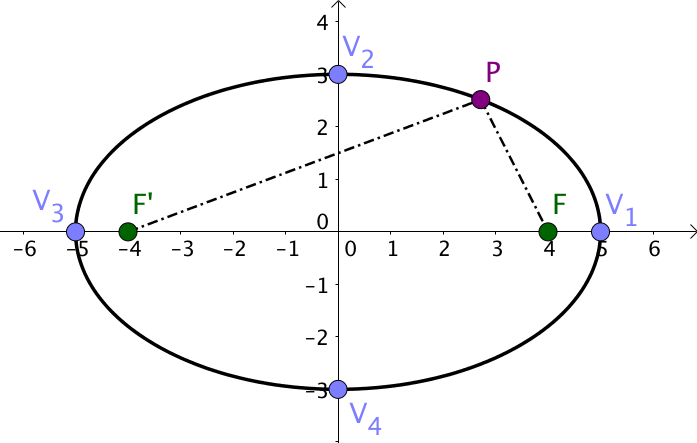
\includegraphics[width=0.9\textwidth]{img-sol/construccio-ellipse}
		
		\ggblink{https://www.geogebra.org/m/yEZzBKCS}
		
		
	\end{center}
\end{minipage}		

	Expressam les distàncies en components
	\[
		\sqrt{(x-4)^2+y^2} + \sqrt{(x+4)^2+y^2}=10
	\]	
	Aïllam la primera arrel i elevam al quadrat els dos membres
	\[
		(x-4)^2+y^2 = 100 +(x+4)^2+y^2 - 20\sqrt{(x+4)^2+y^2}
	\]	
	Tornam a aïllar l'arrel i elevam al quadrat un altre pic
	\[
		-16 x - 100  = - 20\sqrt{(x+4)^2+y^2}
	\]
	\[
		256 x^2 +3200 x + 10000  = 400 \left( (x+4)^2+y^2 \right)
	\]
	Simplificant els quadrats d'aquesta expressió trobam $144x^2+400y^2=3600$, que si dividim tot entre 3600 arribam a
	\[
		\dfrac{x^2}{25}+\dfrac{y^2}{9}=1
	\]
	
	
	
	
	
}


%%% Demostracio hiperbola
\newcommand{\pagecxxxiii}{
	\heading{Exemple construcció hipèrbola}
 \vspace{0.5cm}

	\begin{minipage}{0.5\textwidth}
	
	\textbf{DADES}: Volem trobar l'equació de la hipèrbola que té focus a $F(5,0)$ i $F'(-5,0)$ i té semieix major $a=4$. 
	\vso
	
	El semieix menor es troba de $b=\sqrt{5^2-4^2}=3$.
	
	Per a qualsevol punt $P(x,y)$ sobre la hipèrbola, es compleix que 
	\[
	d(P,F) - d(P,F')=\pm 2a= \pm 8
	\]
	
\end{minipage}
\hspace{0.5cm}
\begin{minipage}{0.43\textwidth}
	
	\begin{center}	
		
		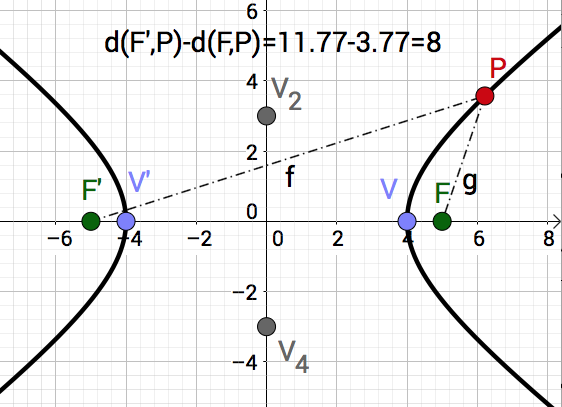
\includegraphics[width=0.9\textwidth]{img-sol/construccio-hiperbola}
		
		\ggblink{https://www.geogebra.org/m/CdRCjv8S}	
		
		
	\end{center}
\end{minipage}		

Expressam les distàncies en components
\[
\sqrt{(x-5)^2+y^2} - \sqrt{(x+5)^2+y^2}=\pm 8
\]	
Aïllam la primera arrel i elevam al quadrat els dos membres
\[
(x-5)^2+y^2 = 64 +(x+5)^2+y^2 + 16\sqrt{(x+5)^2+y^2}
\]	
Tornam a aïllar l'arrel i elevam al quadrat un altre pic
\[
-20 x - 64  =  16\sqrt{(x+5)^2+y^2}
\]
\[
400 x^2 +2560x + 4096  = 256 \left( (x+5)^2+y^2 \right)
\]
Simplificant els quadrats d'aquesta expressió trobam $144x^2-256y^2=2304$, que si dividim tot entre 2304 arribam a
\[
\dfrac{x^2}{16}-\dfrac{y^2}{9}=1
\]

}


%%% Demostracio parabola en general
\newcommand{\pagecxxxiv}{
	\heading{Exemple construcció paràbola obliqua}
 \vspace{0.5cm}

\begin{minipage}{0.5\textwidth}
	
	\textbf{DADES}: Volem trobar l'equació de la paràbola que té focus a $F(2,1)$ i recta directriu $r:\; y=x-5$. 
	\vso
	
	Per a qualsevol punt $A(x,y)$ sobre la paràbola, es compleix que 
	\[
	d(A,F)= d(A,r)
	\]
	
\end{minipage}
\hspace{0.5cm}
\begin{minipage}{0.43\textwidth}
	
	\begin{center}	
		
			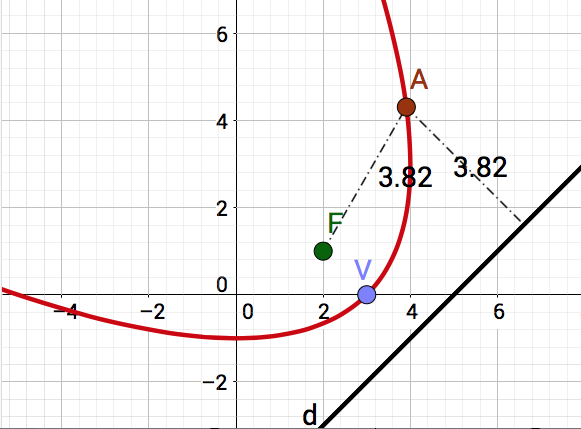
\includegraphics[width=0.9\textwidth]{img-sol/construccio-parabola}
		
			\ggblink{https://www.geogebra.org/m/b6JmdezZ}
		
		
	\end{center}
\end{minipage}	

Expressam les distàncies en components
\[
\sqrt{(x-2)^2+(y-1)^2} = \dfrac{|x-y-5|}{\sqrt{2}}
\]
Elevam al quadrat
\[
(x-2)^2+(y-1)^2 = \dfrac{(x-y-5)^2}{2}
\]
Multiplicam per tot i desenvolupam els quadrats:
\[
	2\left[ x^2-2x+4 +y^2-2y+1 \right] = x^2+y^2 -2xy -10x+10y+25
\]
Simplificant, arribam a l'equació de la paràbola obliqua:
\[
	x^2+y^2+2xy+2x-14y-15=0
\] 
}



%%% estadistica 1d
\newcommand{\pagecxlii}{
	
	\heading{Distribucions marginals}
	
	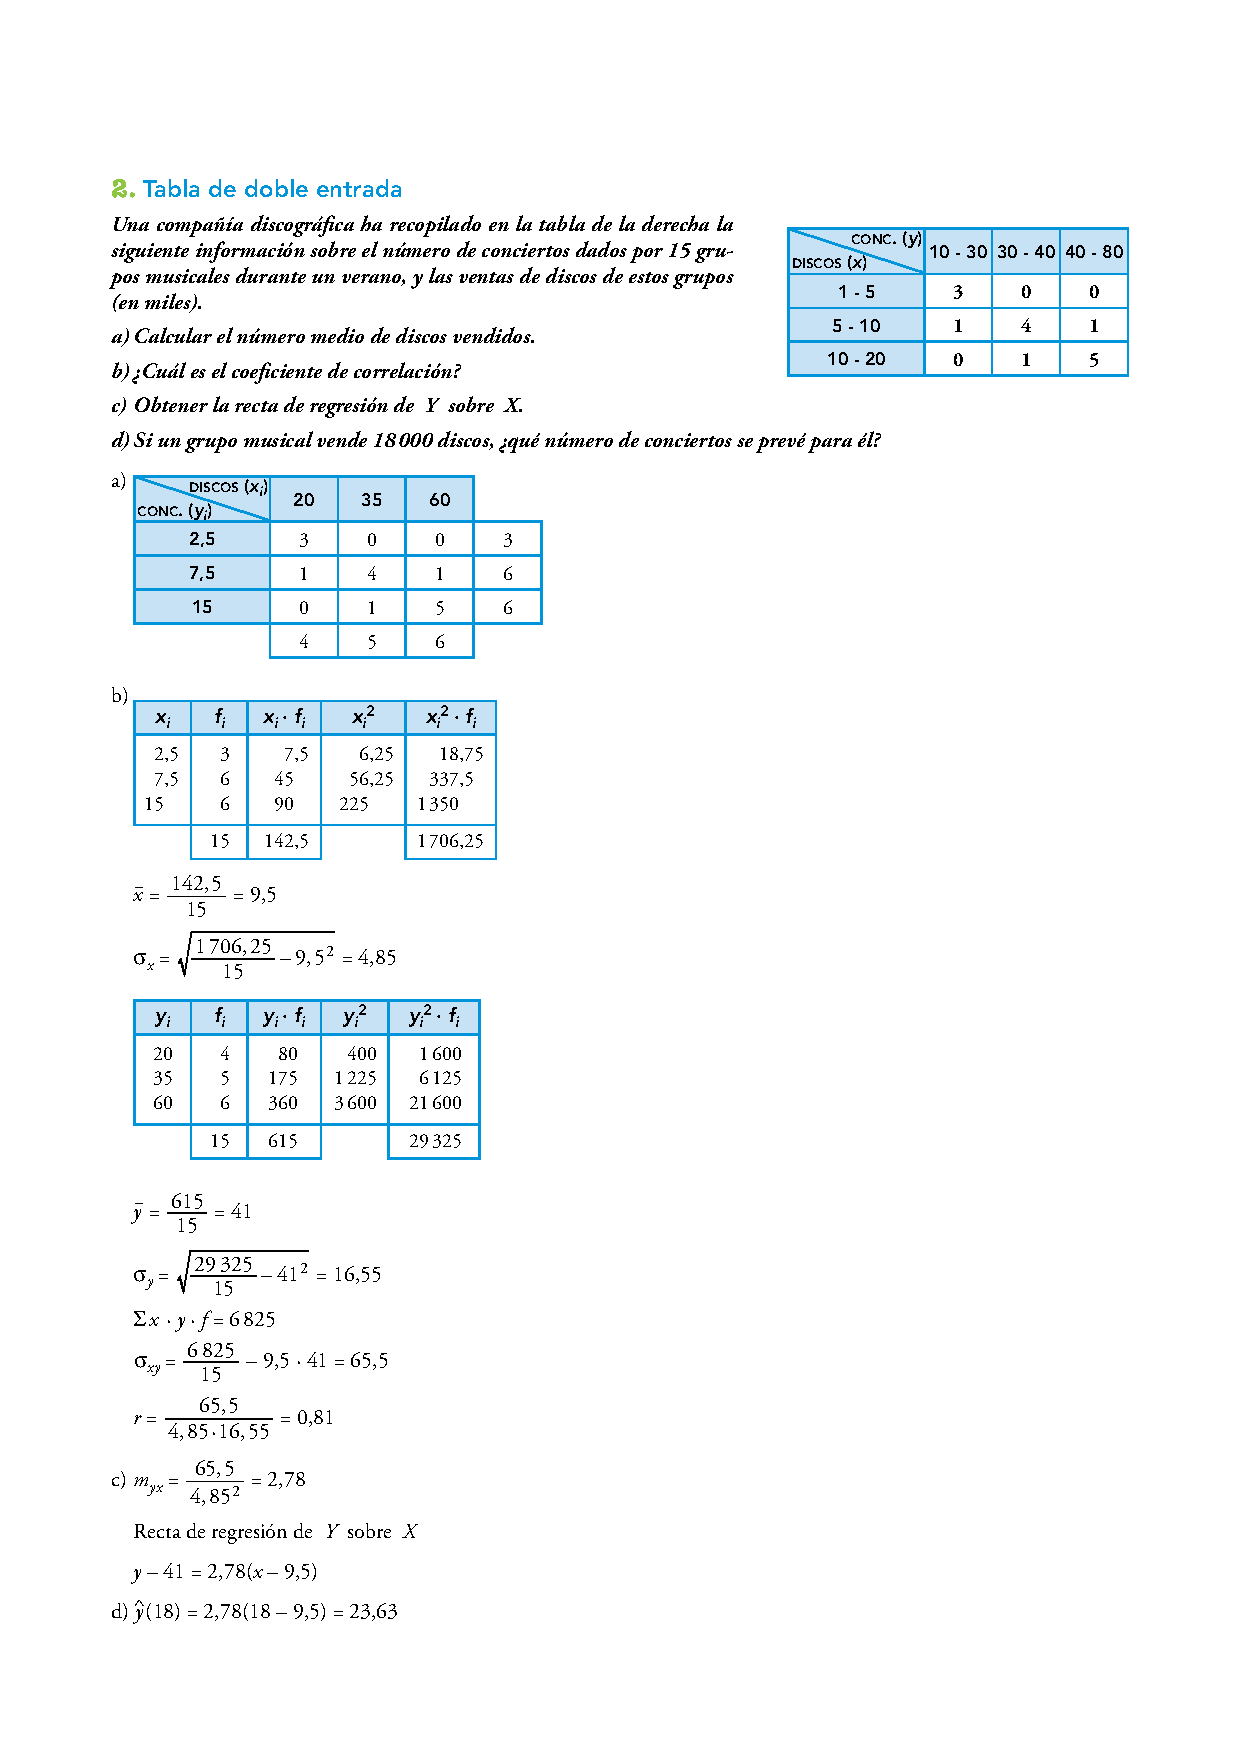
\includegraphics[width=\textwidth]{img-sol/p147-extra}
}


%%% estadistica nuvols i bimbolles
\newcommand{\pagecxlv}{
	
	\heading{Núvols de punts}
	
	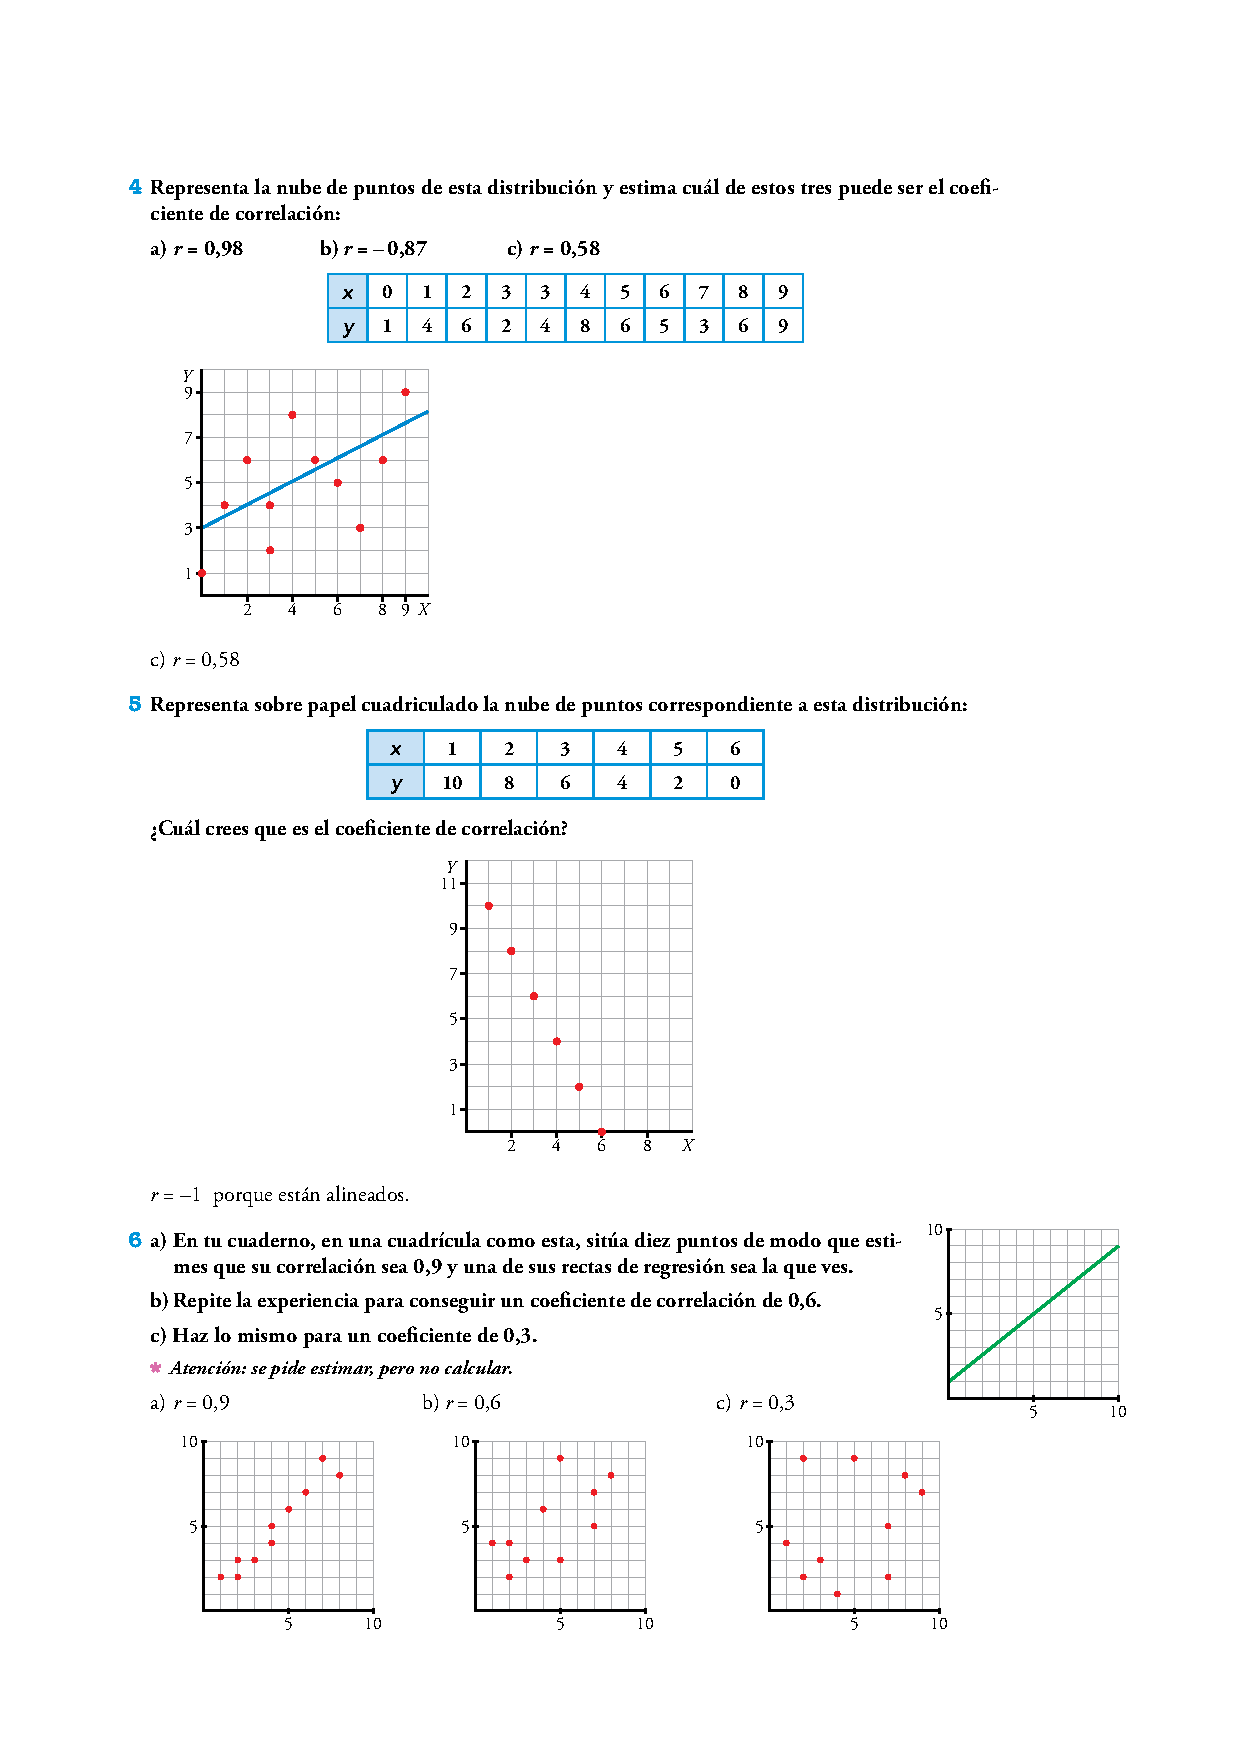
\includegraphics[width=\textwidth]{img-sol/p145-extra}
}


%%% estadistica: coeficent amb dades agrupades
\newcommand{\pagecxlvii}{
	
	\heading{Càlcul de $r$ amb dades agrupades}
	
	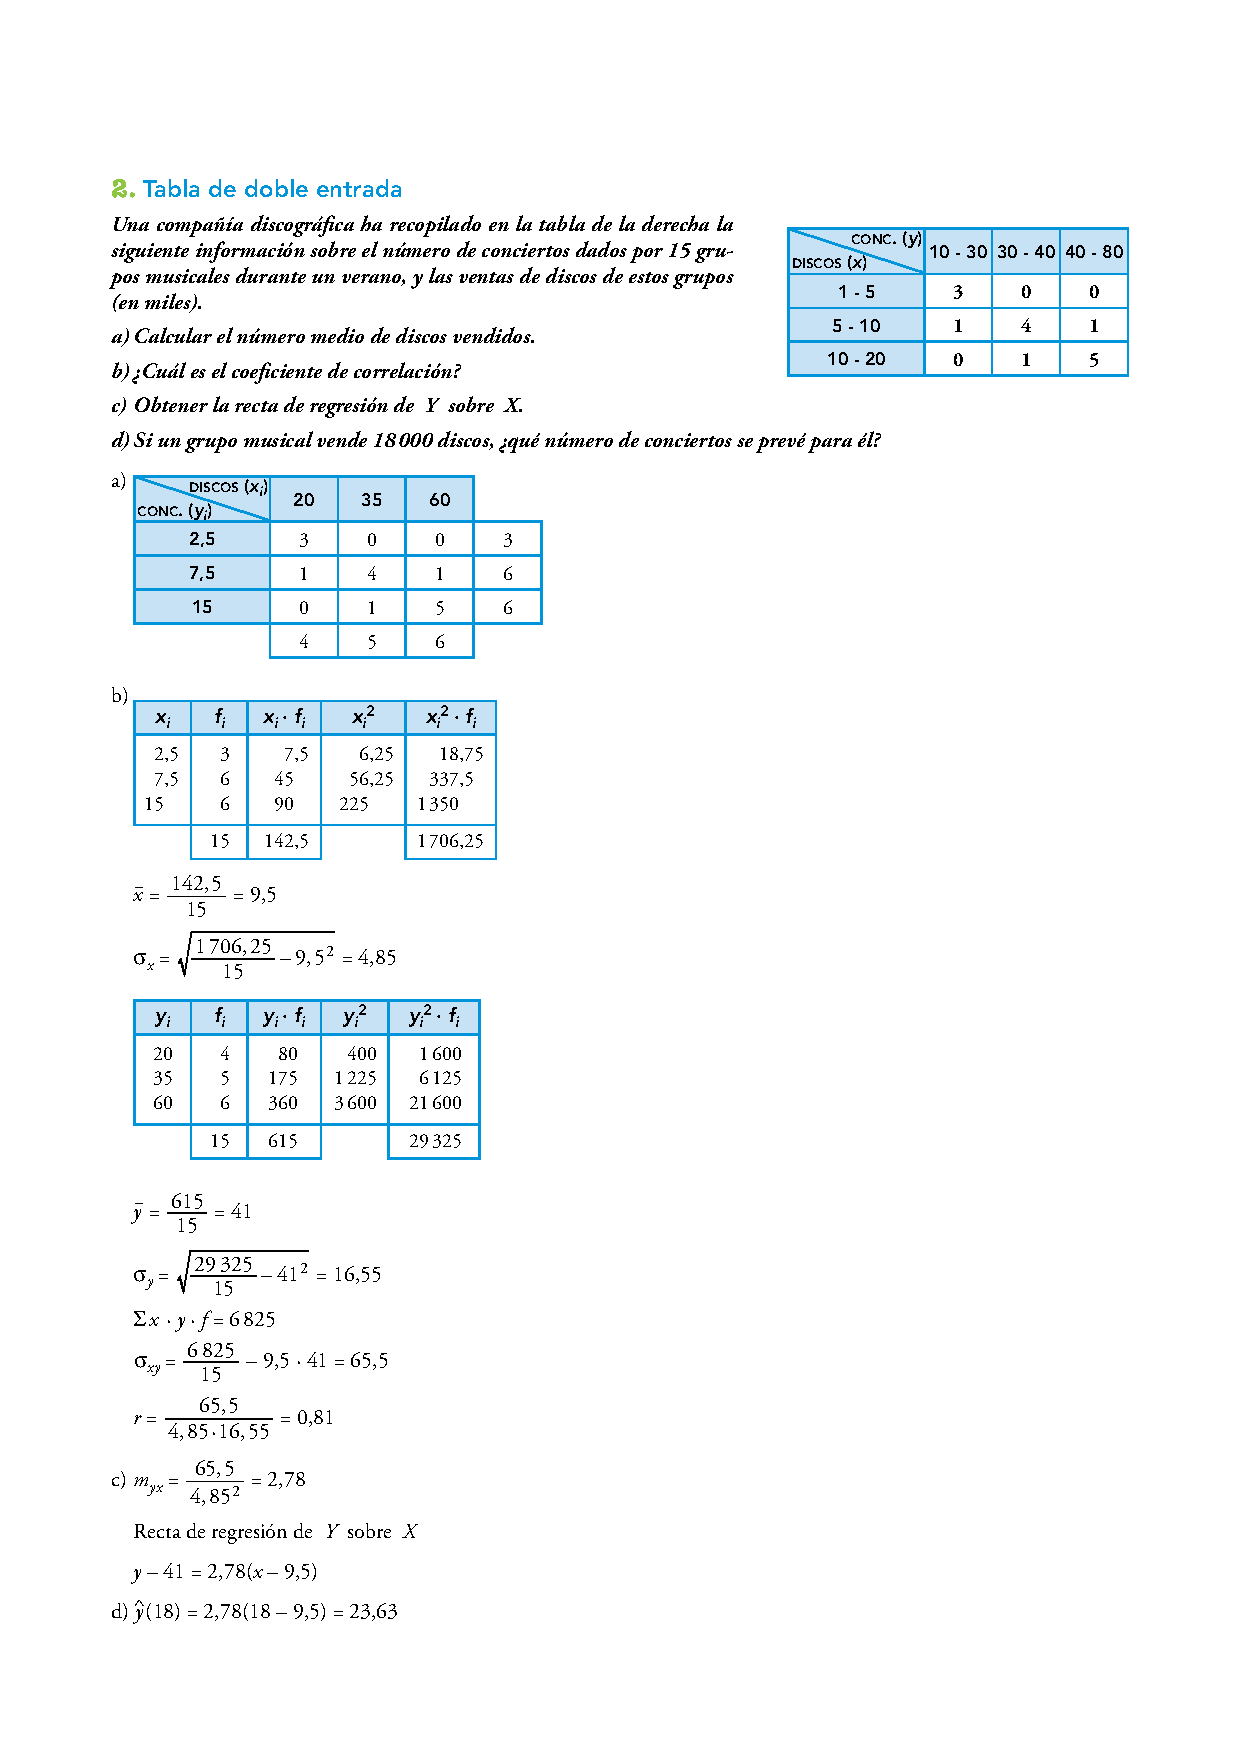
\includegraphics[width=\textwidth]{img-sol/p147-extra}
}


\newcommand{\pagecxlviii}{
	
	\heading{Recta X sobre Y}
	
	Si volem fer una predicció conegut el valor de $y$  trobar el valor de $x$, podem utilitzar l'equació de la recta de regressió $y=\bar y + \dfrac{\sigma_{xy}}{\sigma_x^2} (x-\bar x)$ i aïllar el valor de $x$.
	
	El més lògic, però és utilitzar la recta de regressió X sobre Y
	\[ x=\bar x + \dfrac{\sigma_{xy}}{\sigma_y^2} (y-\bar y) \]
	que ja ens proporcionarà directament el valor de $x$ conegut $y$.
	
	Cal assenyalar que quan $|r|\rightarrow 1$, les dues prediccions seran pràcticament iguals. Per correlacions febles, obtindrem valors molt distints, cosa que indica que la predicció és poc fiable.
}

